\documentclass{article}\usepackage[]{graphicx}\usepackage[]{color}
%% maxwidth is the original width if it is less than linewidth
%% otherwise use linewidth (to make sure the graphics do not exceed the margin)
\makeatletter
\def\maxwidth{ %
  \ifdim\Gin@nat@width>\linewidth
    \linewidth
  \else
    \Gin@nat@width
  \fi
}
\makeatother

\definecolor{fgcolor}{rgb}{0.345, 0.345, 0.345}
\newcommand{\hlnum}[1]{\textcolor[rgb]{0.686,0.059,0.569}{#1}}%
\newcommand{\hlstr}[1]{\textcolor[rgb]{0.192,0.494,0.8}{#1}}%
\newcommand{\hlcom}[1]{\textcolor[rgb]{0.678,0.584,0.686}{\textit{#1}}}%
\newcommand{\hlopt}[1]{\textcolor[rgb]{0,0,0}{#1}}%
\newcommand{\hlstd}[1]{\textcolor[rgb]{0.345,0.345,0.345}{#1}}%
\newcommand{\hlkwa}[1]{\textcolor[rgb]{0.161,0.373,0.58}{\textbf{#1}}}%
\newcommand{\hlkwb}[1]{\textcolor[rgb]{0.69,0.353,0.396}{#1}}%
\newcommand{\hlkwc}[1]{\textcolor[rgb]{0.333,0.667,0.333}{#1}}%
\newcommand{\hlkwd}[1]{\textcolor[rgb]{0.737,0.353,0.396}{\textbf{#1}}}%
\let\hlipl\hlkwb

\usepackage{framed}
\makeatletter
\newenvironment{kframe}{%
 \def\at@end@of@kframe{}%
 \ifinner\ifhmode%
  \def\at@end@of@kframe{\end{minipage}}%
  \begin{minipage}{\columnwidth}%
 \fi\fi%
 \def\FrameCommand##1{\hskip\@totalleftmargin \hskip-\fboxsep
 \colorbox{shadecolor}{##1}\hskip-\fboxsep
     % There is no \\@totalrightmargin, so:
     \hskip-\linewidth \hskip-\@totalleftmargin \hskip\columnwidth}%
 \MakeFramed {\advance\hsize-\width
   \@totalleftmargin\z@ \linewidth\hsize
   \@setminipage}}%
 {\par\unskip\endMakeFramed%
 \at@end@of@kframe}
\makeatother

\definecolor{shadecolor}{rgb}{.97, .97, .97}
\definecolor{messagecolor}{rgb}{0, 0, 0}
\definecolor{warningcolor}{rgb}{1, 0, 1}
\definecolor{errorcolor}{rgb}{1, 0, 0}
\newenvironment{knitrout}{}{} % an empty environment to be redefined in TeX

\usepackage{alltt}
\usepackage[utf8]{inputenc}
\usepackage{hyperref}
\hypersetup{
    linktocpage,
    colorlinks=true, 
    linkcolor=blue,
    citecolor=blue,
    filecolor=blue,
    urlcolor=blue
}
\IfFileExists{upquote.sty}{\usepackage{upquote}}{}
\begin{document}


\title{Transcription vs Metilation}
\author{Lucas Michel Todó}
\maketitle
\tableofcontents
\clearpage


%------------------------------------------------------------------------------------------------------------------------------------------
%---------------------------------------------------------INTRO----------------------------------------------------------------------------




%------------------------------------------------------------------------------------------------------------------------------------------
%-------------------------------------------------FILTRATS PER TRANSCRIPCIÓ----------------------------------------------------------------

\section{Heatmaps filtrats i ordenats per Transcripció}
\subsection{Percentatge de gen covert}
\begin{knitrout}
\definecolor{shadecolor}{rgb}{0.969, 0.969, 0.969}\color{fgcolor}\begin{kframe}
\begin{verbatim}
## [1] "erythrocyte membrane protein 1%2C PfEMP1"
## [1] "Plasmodium exported protein (PHISTa)%2C unknown function"
## [1] "cytoadherence linked asexual protein 2"
## [1] "rifin"
## [1] "rifin"
## [1] "rifin"
## [1] "cytoadherence linked asexual protein 3.1"
## [1] "Plasmodium exported protein (PHISTa)%2C unknown function"
## [1] "Plasmodium exported protein%2C unknown function"
## [1] "procollagen lysine 5-dioxygenase%2C putative"
## [1] "rifin%2C pseudogene"
## [1] "rifin"
## [1] "rifin"
## [1] "Pfmc-2TM Maurer's cleft two transmembrane protein"
## [1] "rifin"
## [1] "conserved Plasmodium protein%2C unknown function"
## [1] "erythrocyte membrane protein 1%2C PfEMP1"
## [1] "merozoite surface protein 4"
## [1] "erythrocyte membrane protein 1%2C PfEMP1"
## [1] "conserved Plasmodium protein%2C unknown function"
## [1] "early transcribed membrane protein 12"
## [1] NA
## [1] "rifin"
## [1] "rifin"
## [1] "DnaJ protein%2C putative"
## [1] NA
## [1] "Plasmodium exported protein (hyp8)%2C unknown function"
## [1] "erythrocyte binding antigen-140"
## [1] "rifin"
## [1] "cytoadherence linked asexual protein 3.2"
\end{verbatim}
\end{kframe}

{\centering 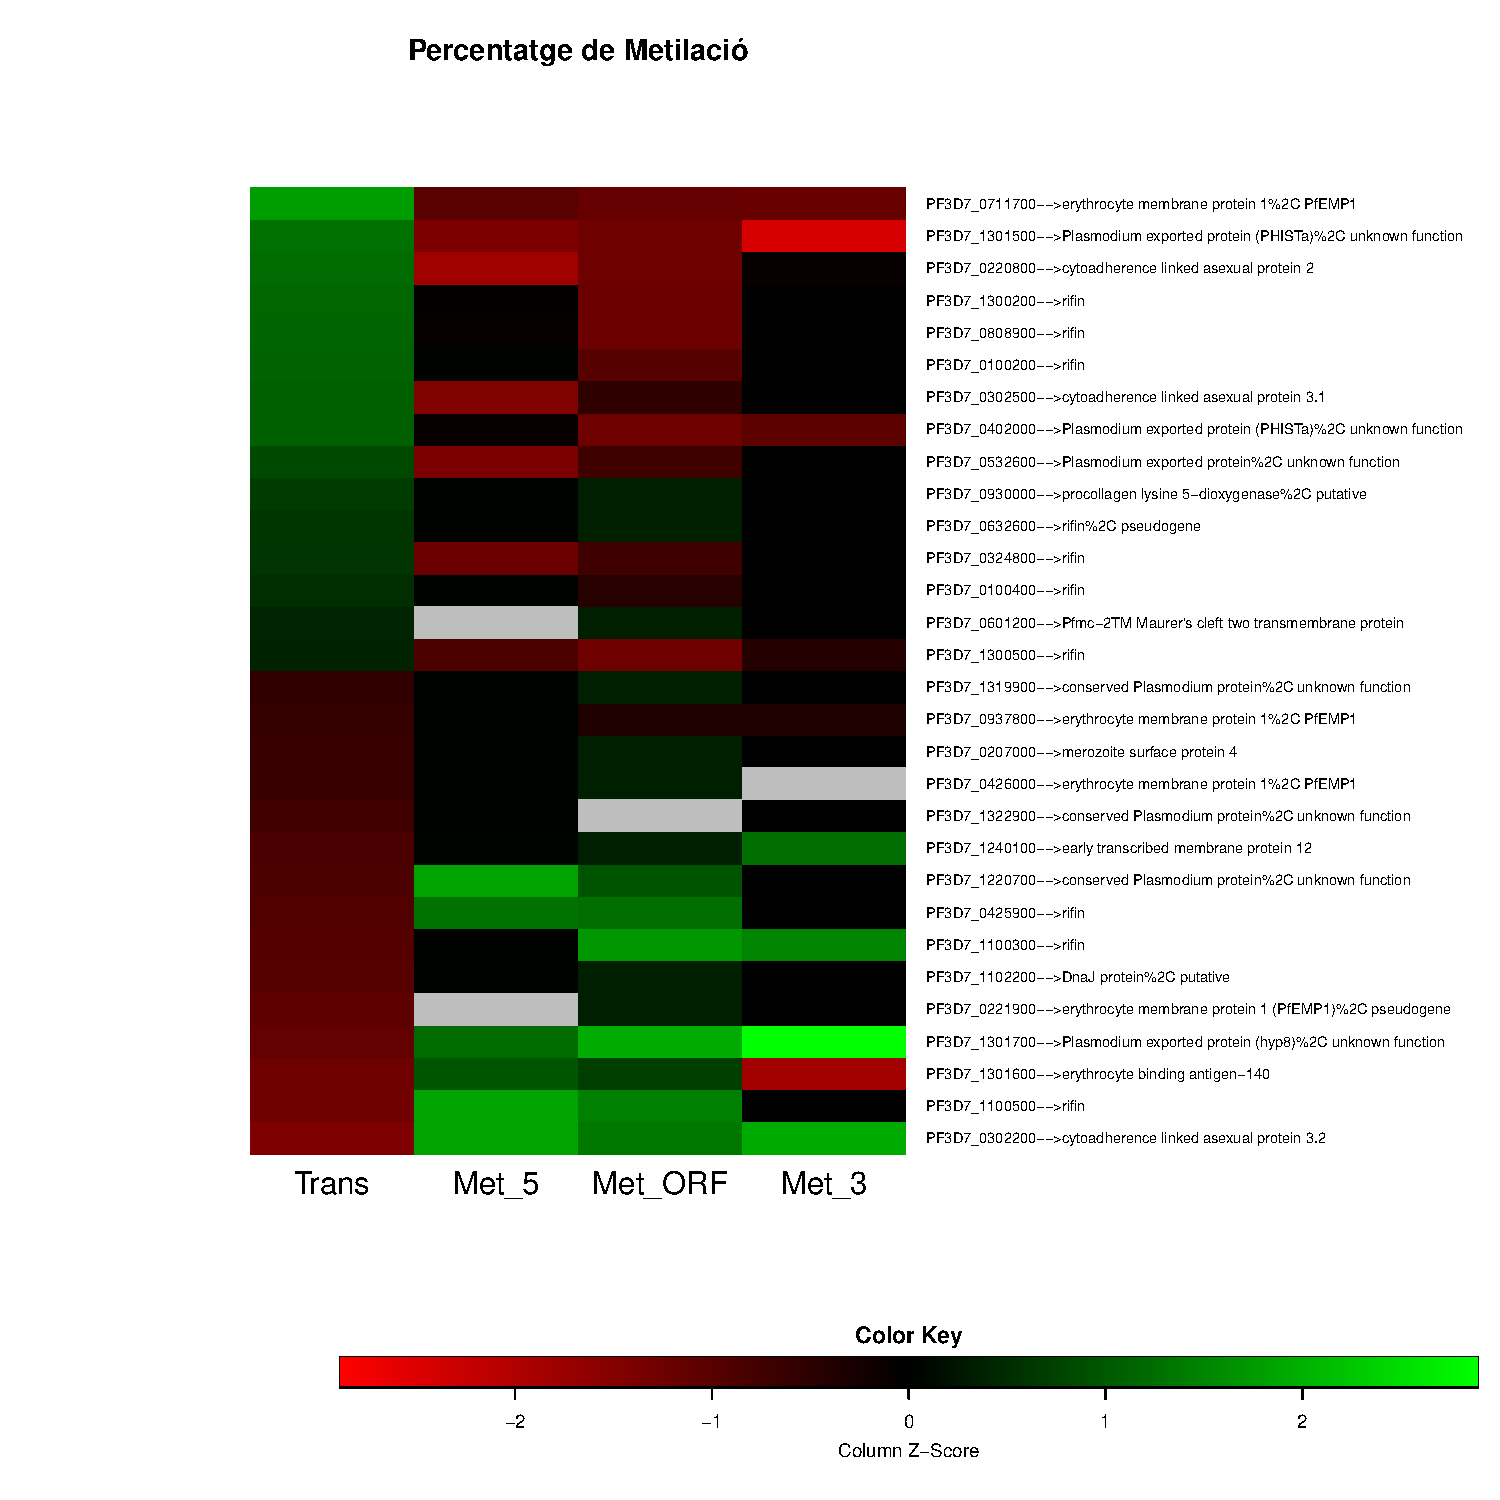
\includegraphics[width=.9\linewidth]{figure/minimal-trans_percent-1} 

}



\end{knitrout}
\clearpage
\subsection{Coverage}
\begin{knitrout}
\definecolor{shadecolor}{rgb}{0.969, 0.969, 0.969}\color{fgcolor}

{\centering 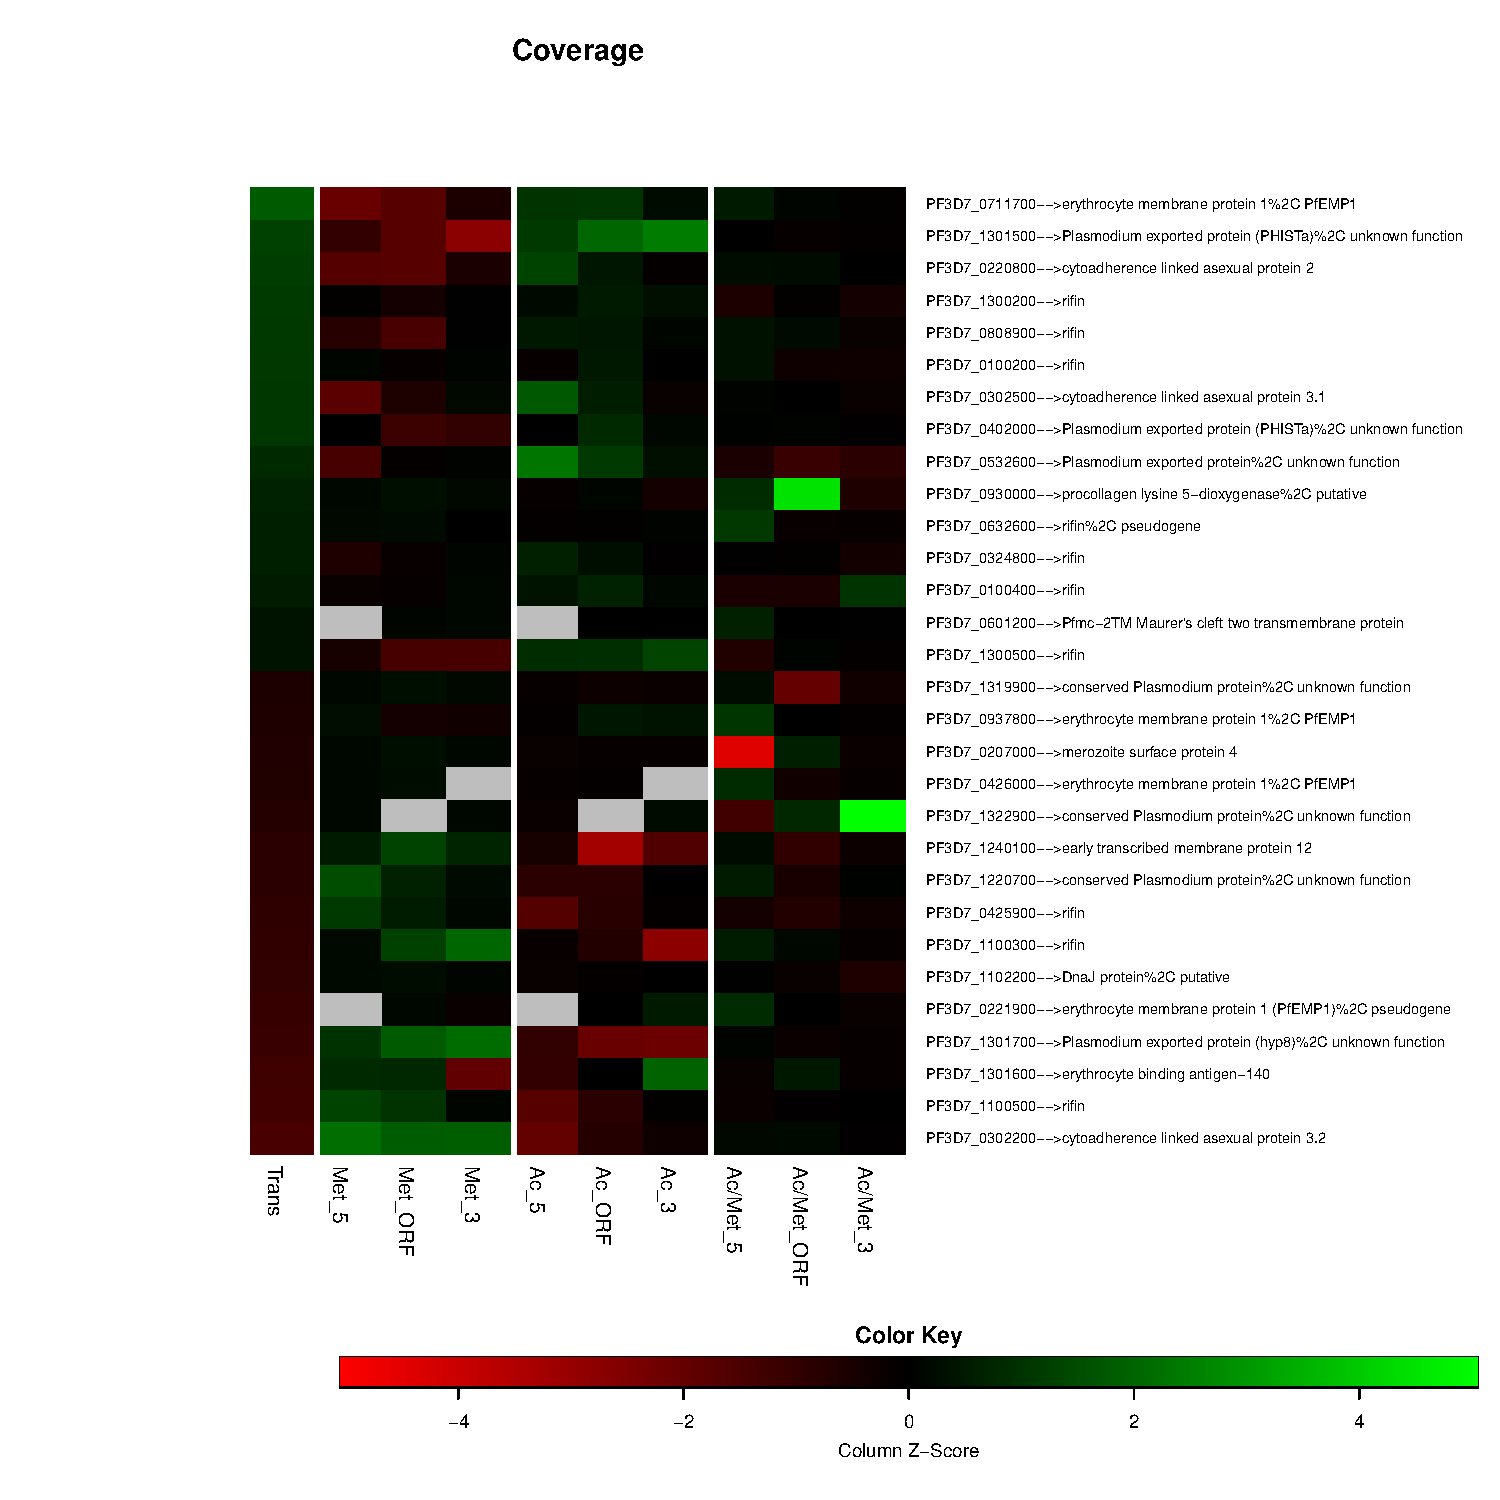
\includegraphics[width=.9\linewidth]{figure/minimal-trans_cov-1} 

}



\end{knitrout}
\clearpage
\subsection{Coverage en Pics}
\begin{knitrout}
\definecolor{shadecolor}{rgb}{0.969, 0.969, 0.969}\color{fgcolor}

{\centering 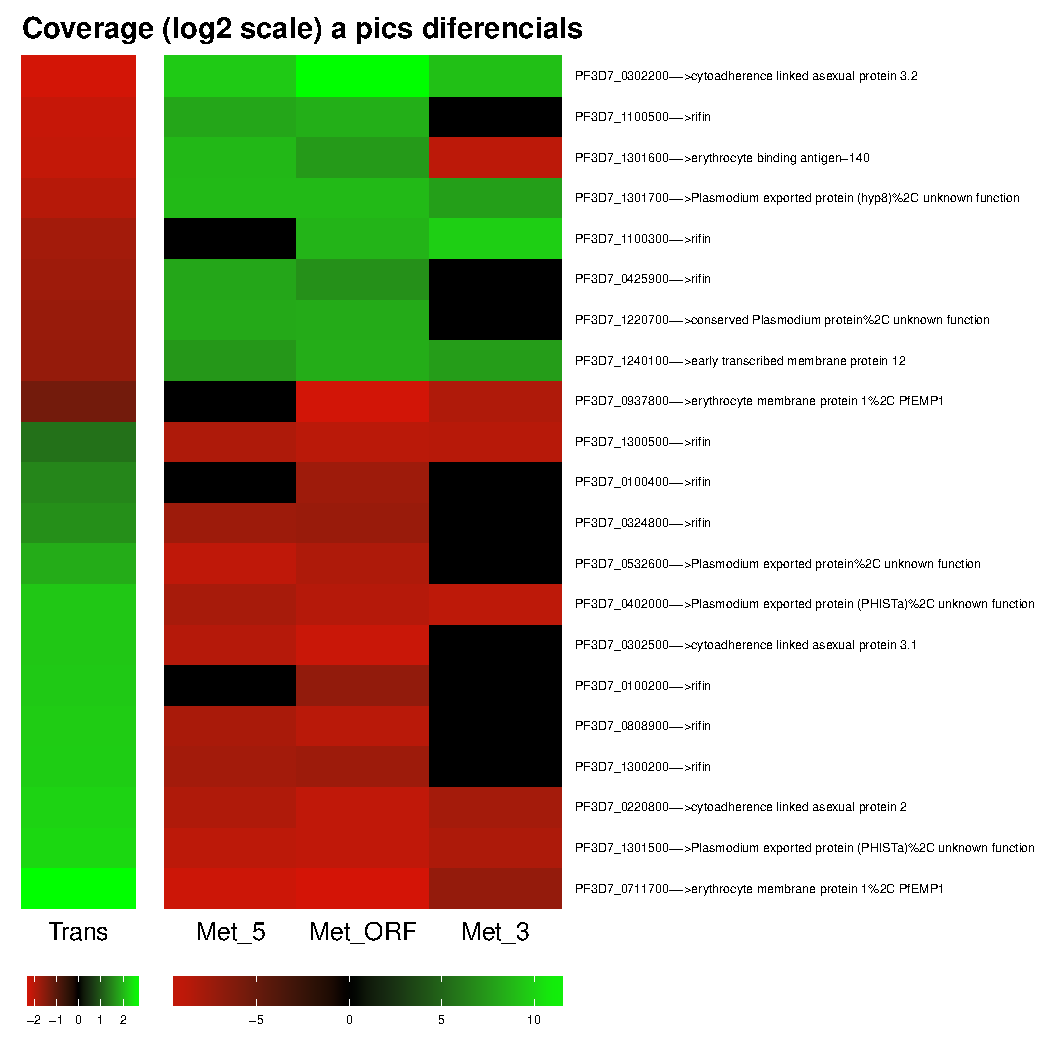
\includegraphics[width=.9\linewidth]{figure/minimal-trans_covapics-1} 

}



\end{knitrout}
\clearpage

%------------------------------------------------------------------------------------------------------------------------------------------
%-------------------------------------------------FILTRATS PER METILACIÓ-------------------------------------------------------------------

\section{Heatmaps filtrats i ordenats per Metilació}
\subsection{Percentatge de gen covert}
\subsubsection{Percentatge de gen covert 5}
\begin{knitrout}
\definecolor{shadecolor}{rgb}{0.969, 0.969, 0.969}\color{fgcolor}

{\centering 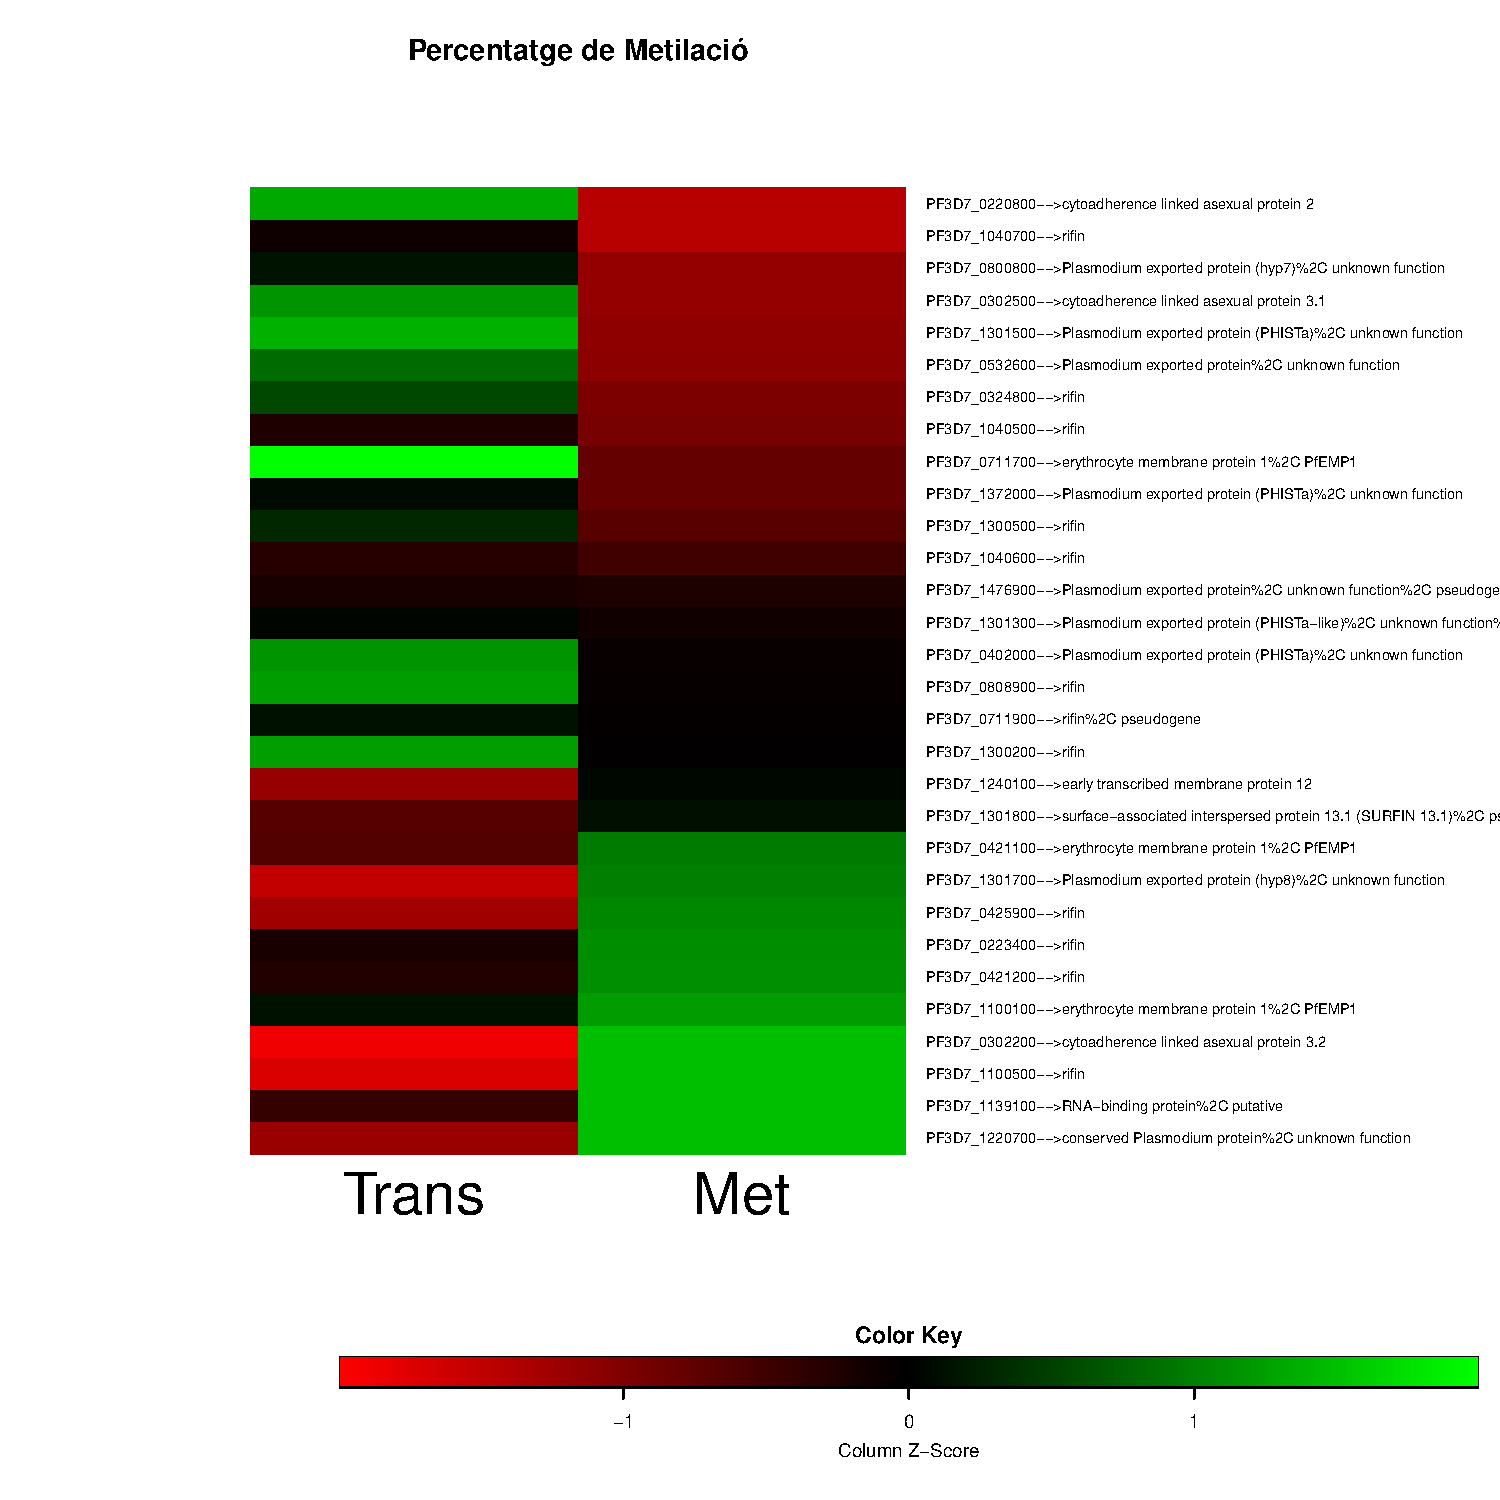
\includegraphics[width=.9\linewidth]{figure/minimal-met_percent_5-1} 

}



\end{knitrout}
\clearpage
\subsubsection{Percentatge de gen covert ORF}
\begin{knitrout}
\definecolor{shadecolor}{rgb}{0.969, 0.969, 0.969}\color{fgcolor}

{\centering 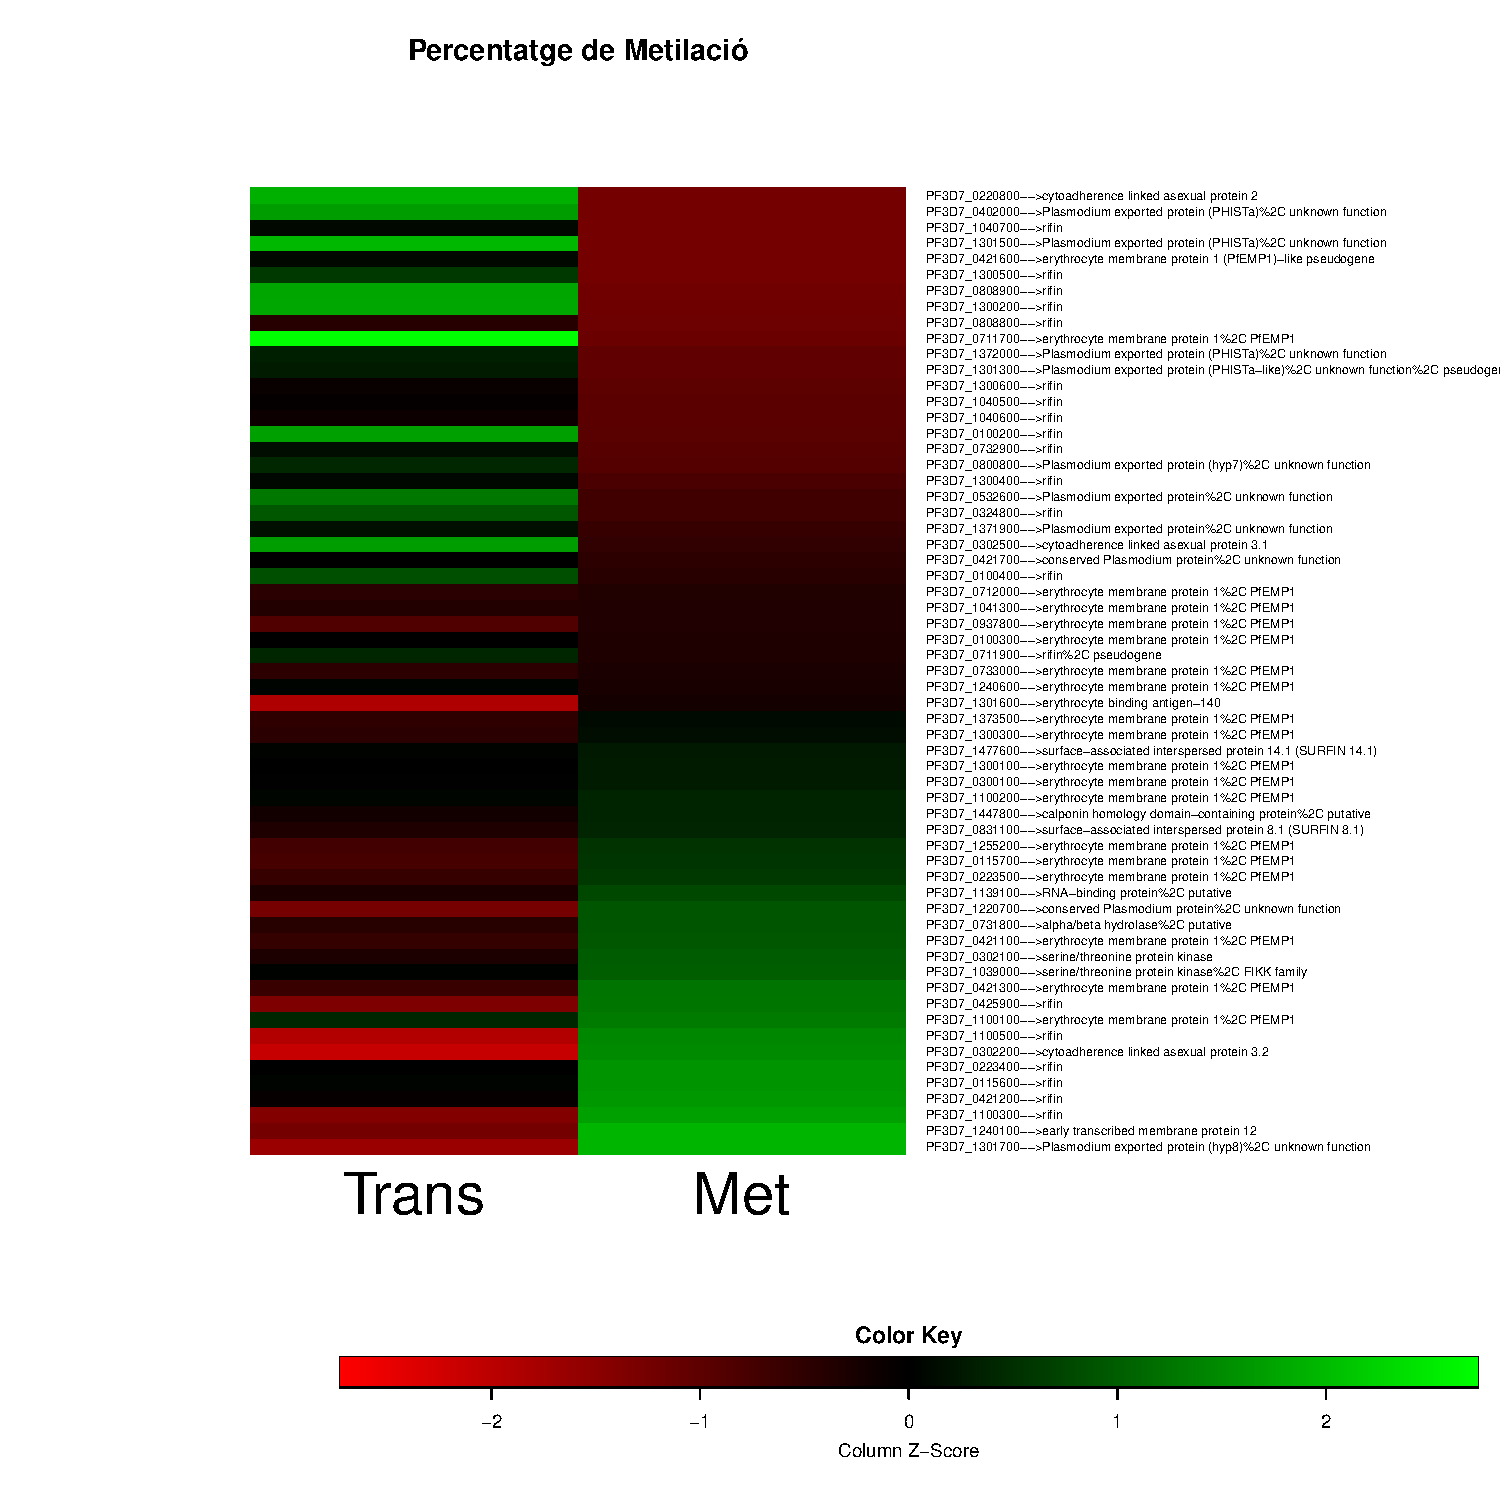
\includegraphics[width=.9\linewidth]{figure/minimal-met_percent_ORF-1} 

}



\end{knitrout}
\clearpage
\subsubsection{Percentatge de gen covert 3}
\begin{knitrout}
\definecolor{shadecolor}{rgb}{0.969, 0.969, 0.969}\color{fgcolor}

{\centering 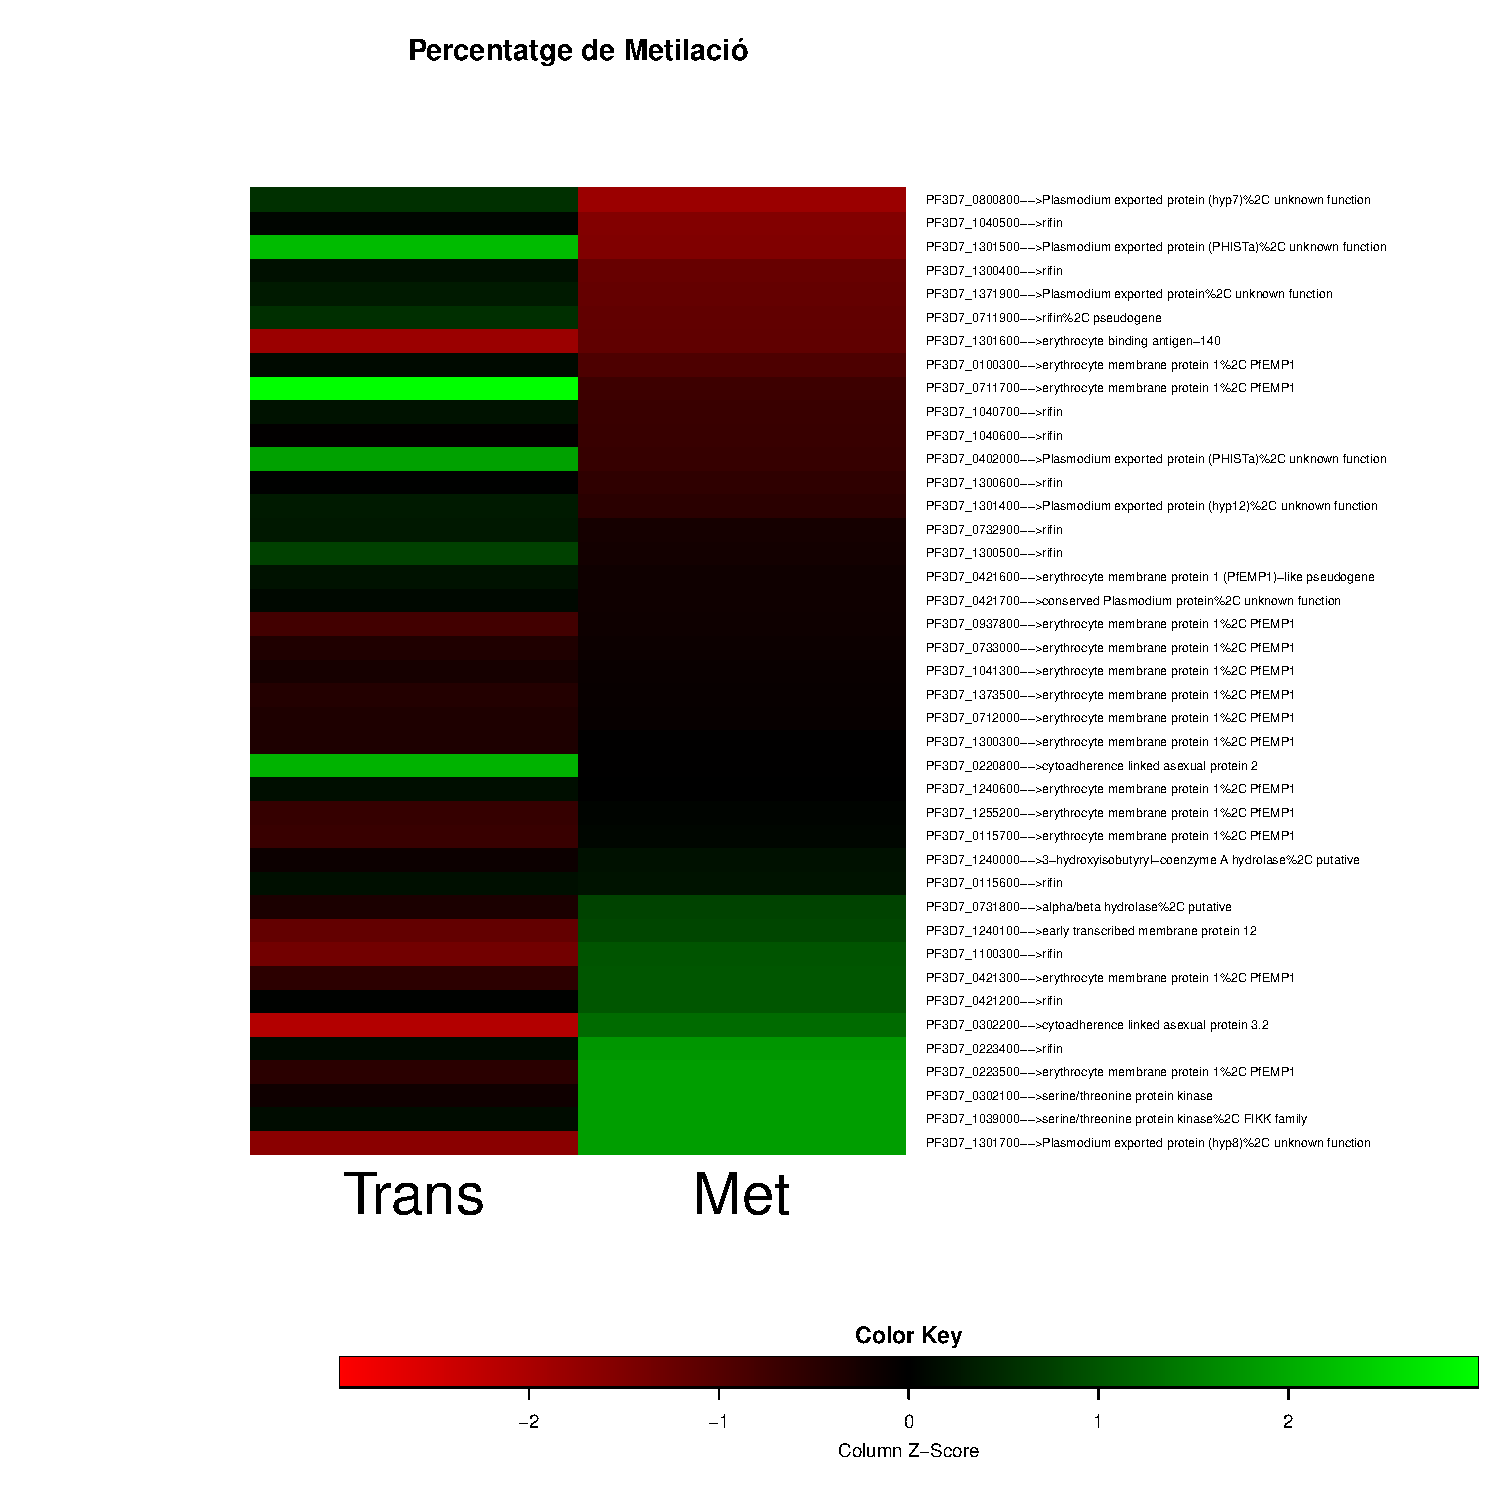
\includegraphics[width=.9\linewidth]{figure/minimal-met_percent_3-1} 

}



\end{knitrout}
\clearpage

\subsection{Coverage}
\subsubsection{Coverage 5}
\begin{knitrout}
\definecolor{shadecolor}{rgb}{0.969, 0.969, 0.969}\color{fgcolor}\begin{kframe}
\begin{verbatim}
## [1] -0.6729804
## [1] -0.7491758
\end{verbatim}
\end{kframe}

{\centering 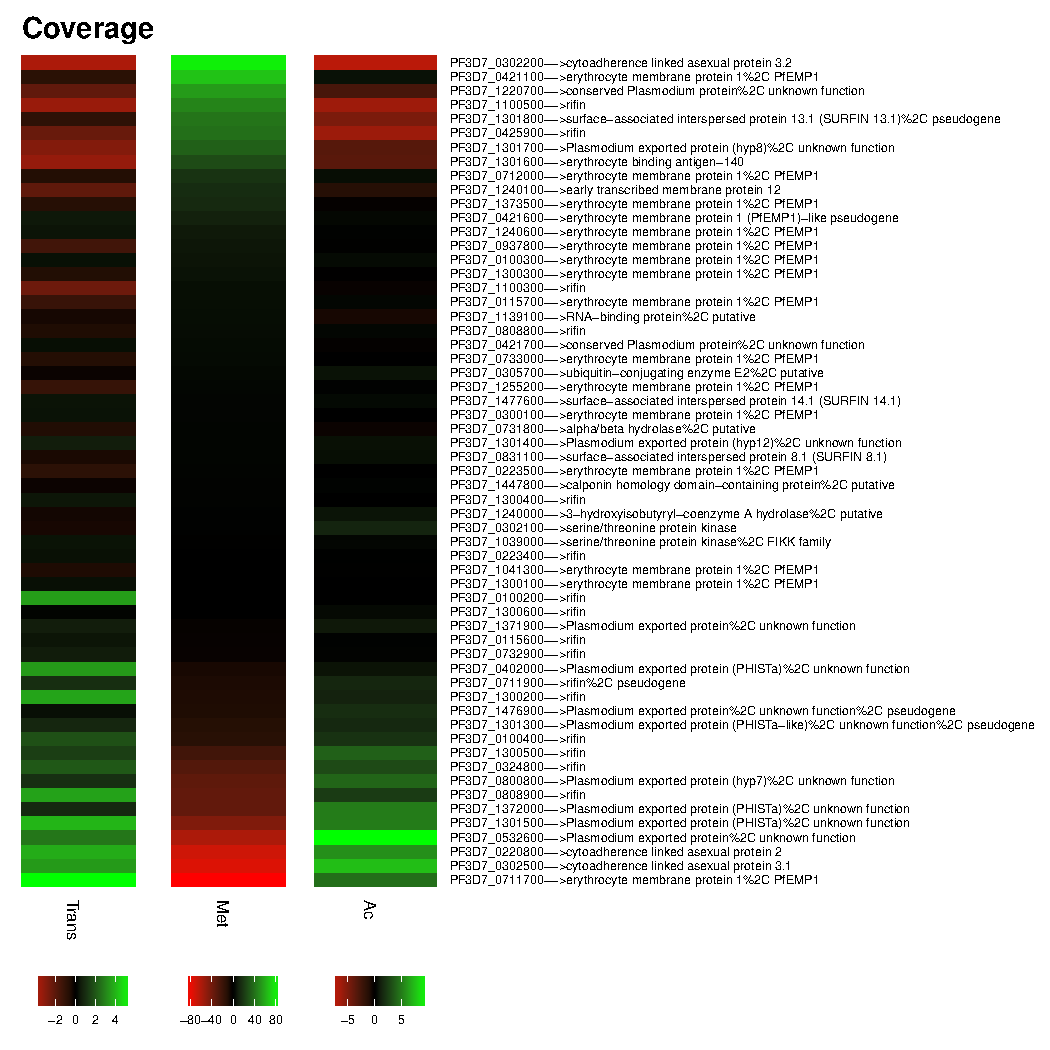
\includegraphics[width=.9\linewidth]{figure/minimal-met_cov_5-1} 

}



\end{knitrout}
\clearpage
\subsubsection{Coverage ORF}
\begin{knitrout}
\definecolor{shadecolor}{rgb}{0.969, 0.969, 0.969}\color{fgcolor}\begin{kframe}
\begin{verbatim}
## [1] -0.5841501
## [1] -0.5648352
\end{verbatim}
\end{kframe}

{\centering 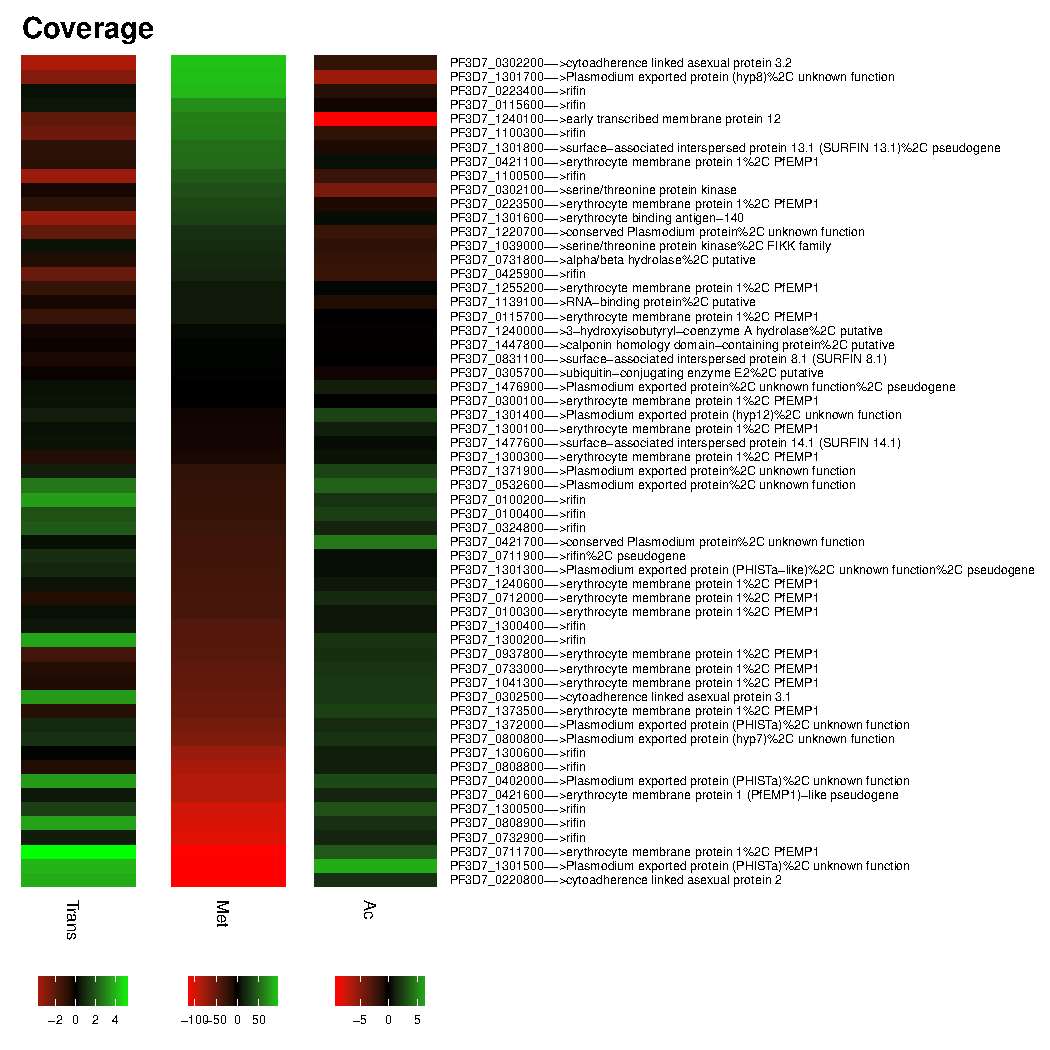
\includegraphics[width=.9\linewidth]{figure/minimal-met_cov_ORF-1} 

}



\end{knitrout}
\clearpage
\subsubsection{Coverage 3}
\begin{knitrout}
\definecolor{shadecolor}{rgb}{0.969, 0.969, 0.969}\color{fgcolor}\begin{kframe}
\begin{verbatim}
## [1] -0.2667113
## [1] -0.3522786
\end{verbatim}
\end{kframe}

{\centering 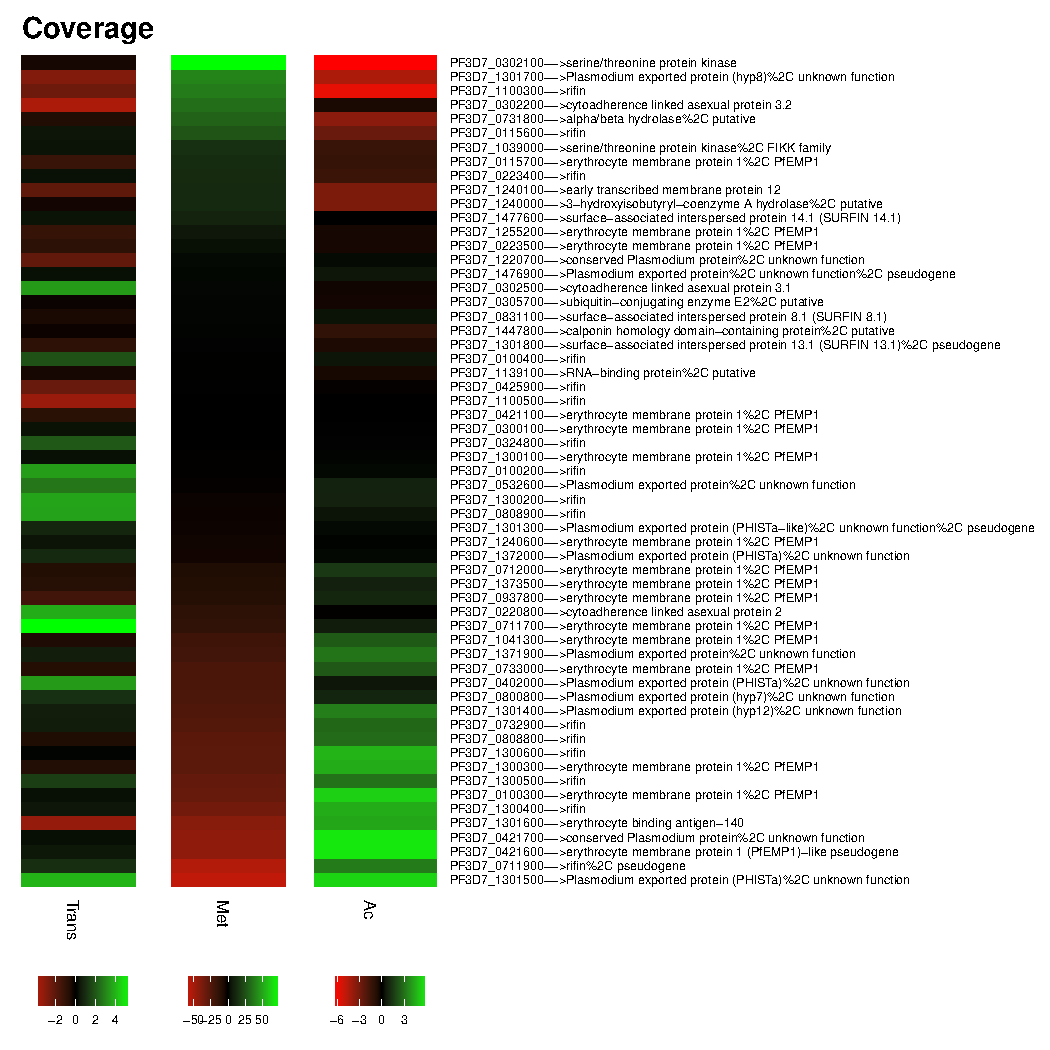
\includegraphics[width=.9\linewidth]{figure/minimal-met_cov_3-1} 

}



\end{knitrout}
\clearpage

\subsection{Coverage en Pics}
S'han exclòs els 0s (gens als quals no hi ha pic a 5'/ORF/3').
\subsubsection{Coverage en Pics 5}
\begin{knitrout}
\definecolor{shadecolor}{rgb}{0.969, 0.969, 0.969}\color{fgcolor}

{\centering 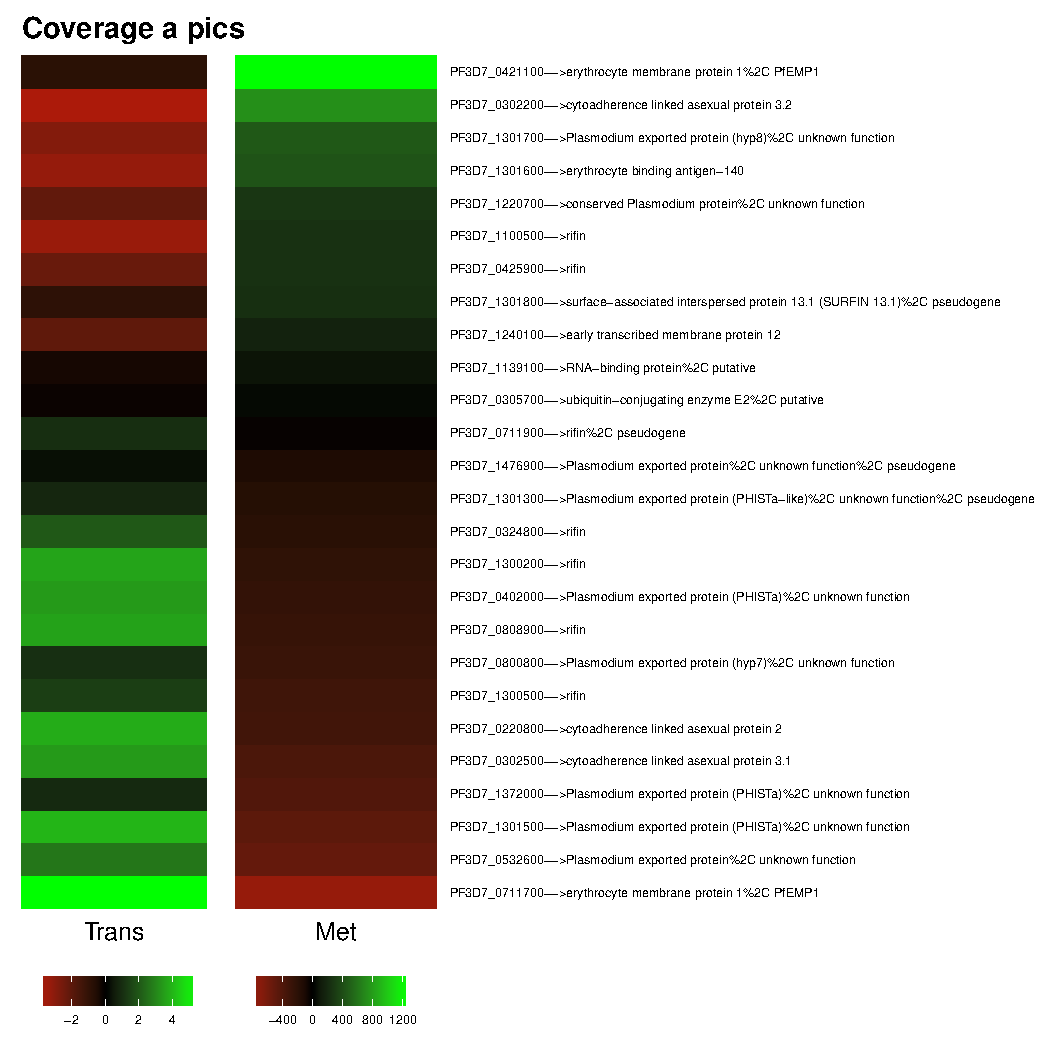
\includegraphics[width=.9\linewidth]{figure/minimal-met_covapics_5-1} 

}



\end{knitrout}
\clearpage
\subsubsection{Coverage en Pics ORF}
\begin{knitrout}
\definecolor{shadecolor}{rgb}{0.969, 0.969, 0.969}\color{fgcolor}

{\centering 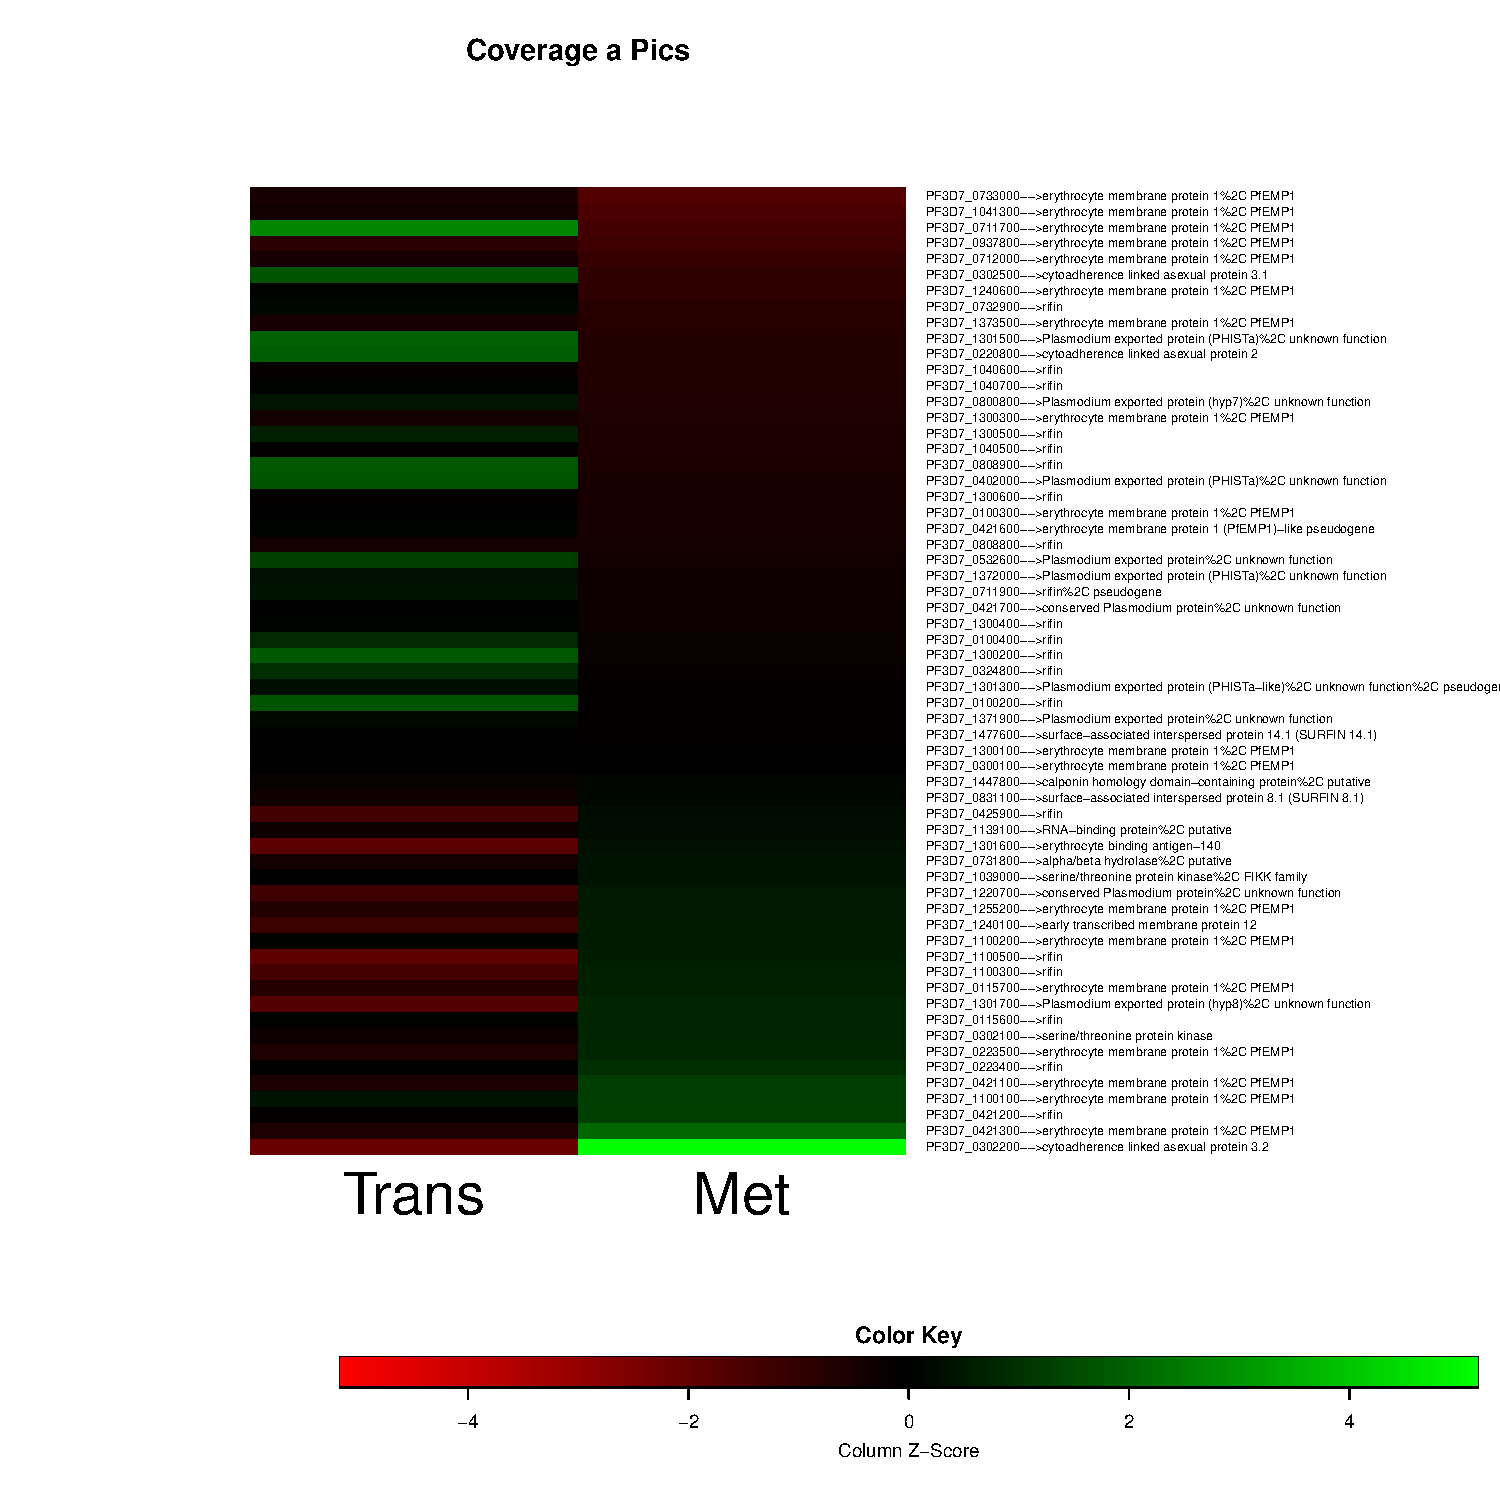
\includegraphics[width=.9\linewidth]{figure/minimal-met_covapics_ORF-1} 

}



\end{knitrout}
\clearpage
\subsubsection{Coverage en Pics 3}
\begin{knitrout}
\definecolor{shadecolor}{rgb}{0.969, 0.969, 0.969}\color{fgcolor}

{\centering 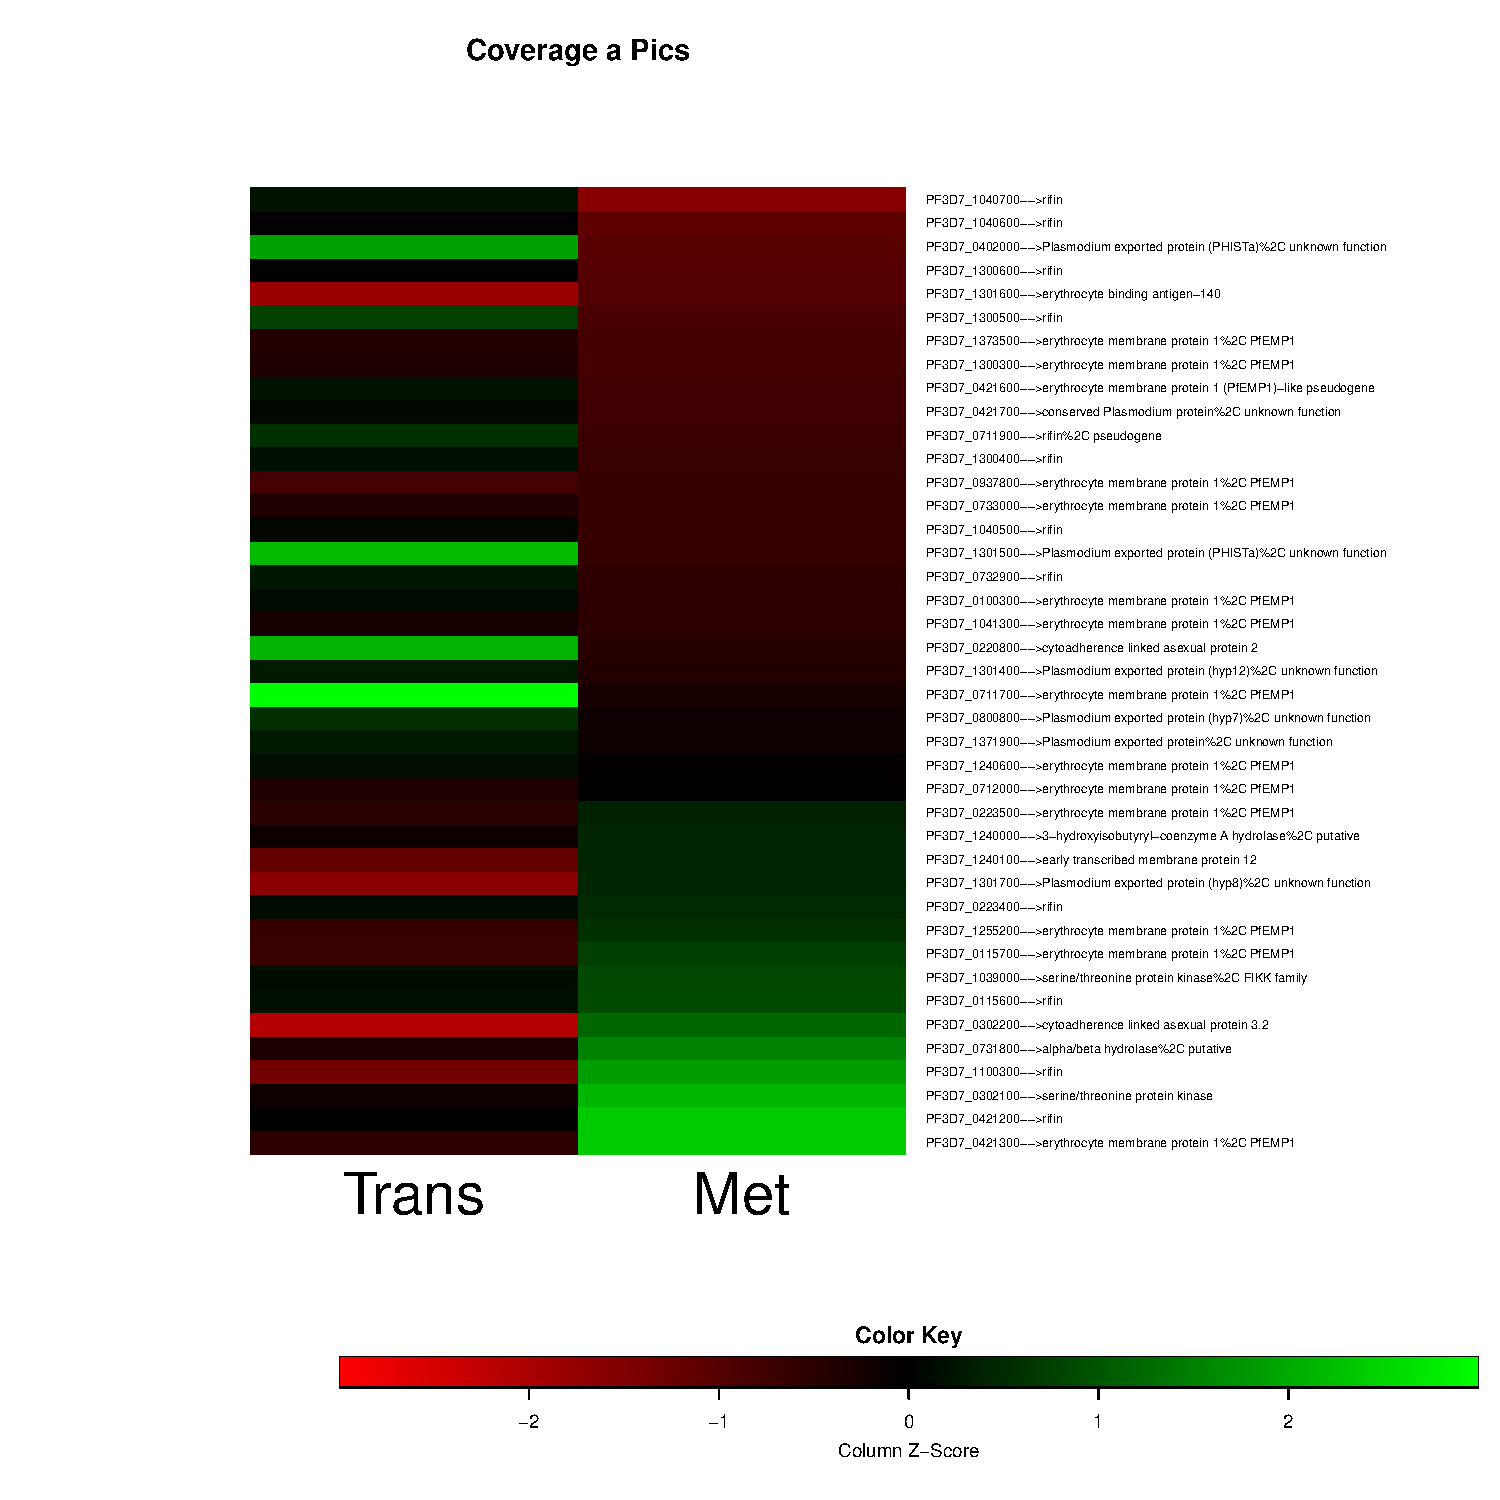
\includegraphics[width=.9\linewidth]{figure/minimal-met_covapics_3-1} 

}



\end{knitrout}
\clearpage


%------------------------------------------------------------------------------------------------------------------------------------------
%-------------------------------------------------CORRELACIONS..........-------------------------------------------------------------------

\section{Anàlisi de correlació}
\subsection{Gràfics}
\subsubsection{Filtrats per Transcripció}
\begin{knitrout}
\definecolor{shadecolor}{rgb}{0.969, 0.969, 0.969}\color{fgcolor}

{\centering 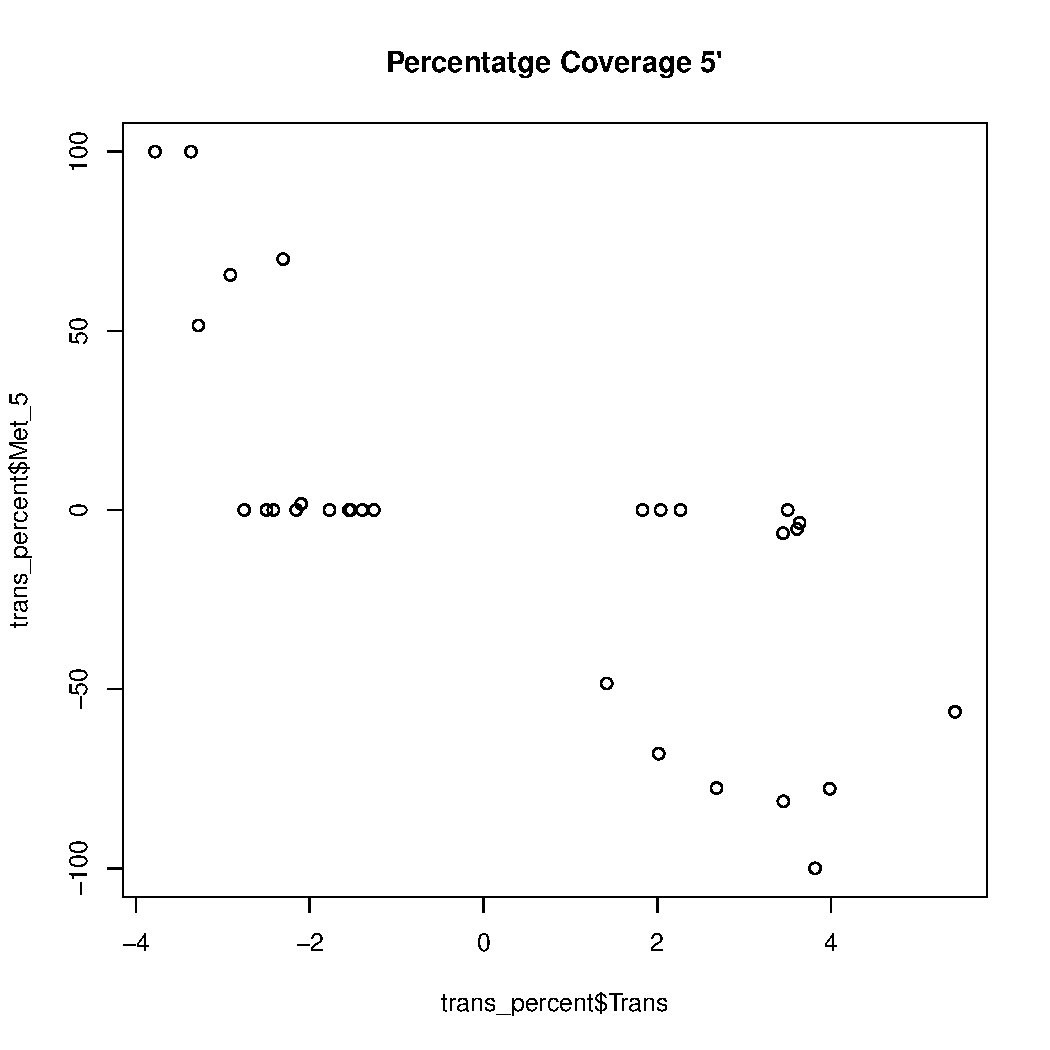
\includegraphics[width=\maxwidth]{figure/minimal-correlacions_trans-1} 
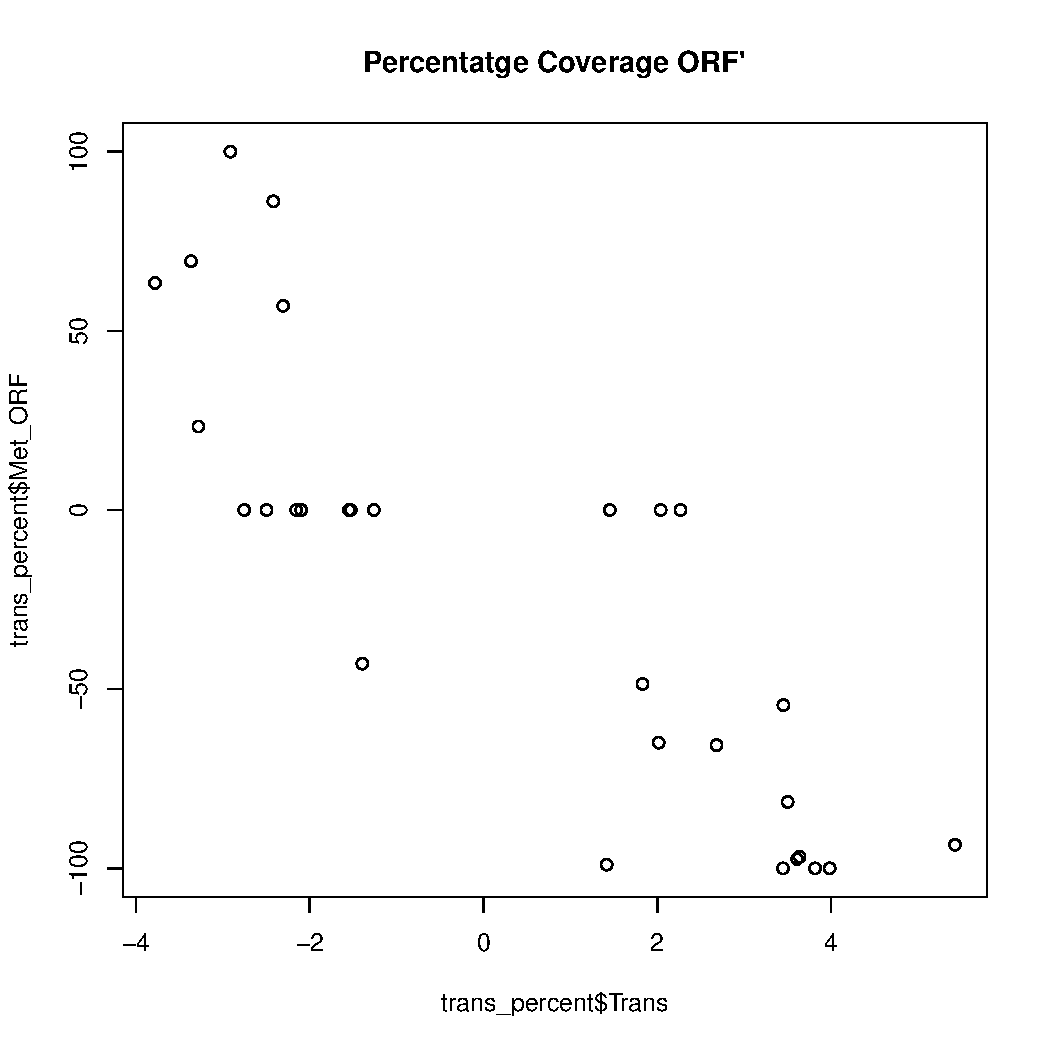
\includegraphics[width=\maxwidth]{figure/minimal-correlacions_trans-2} 
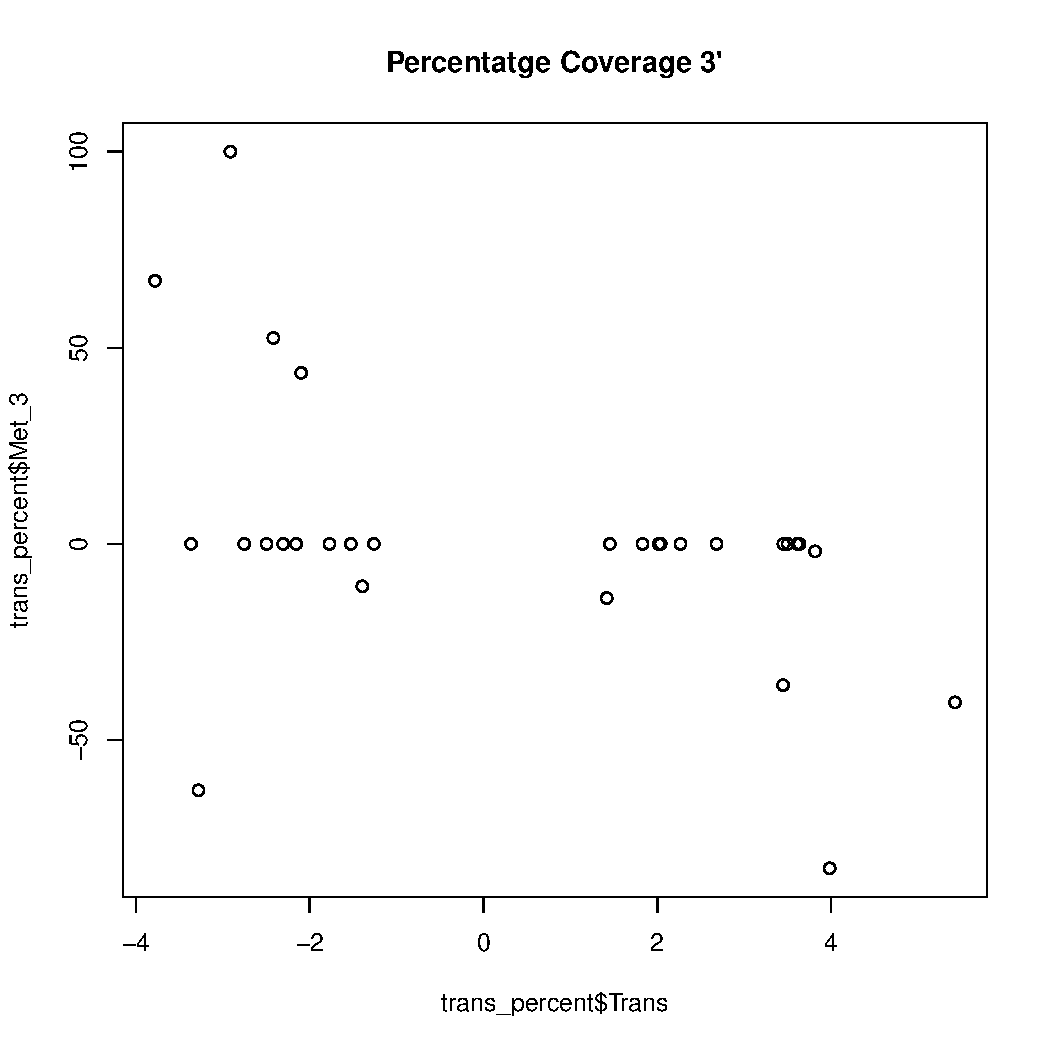
\includegraphics[width=\maxwidth]{figure/minimal-correlacions_trans-3} 
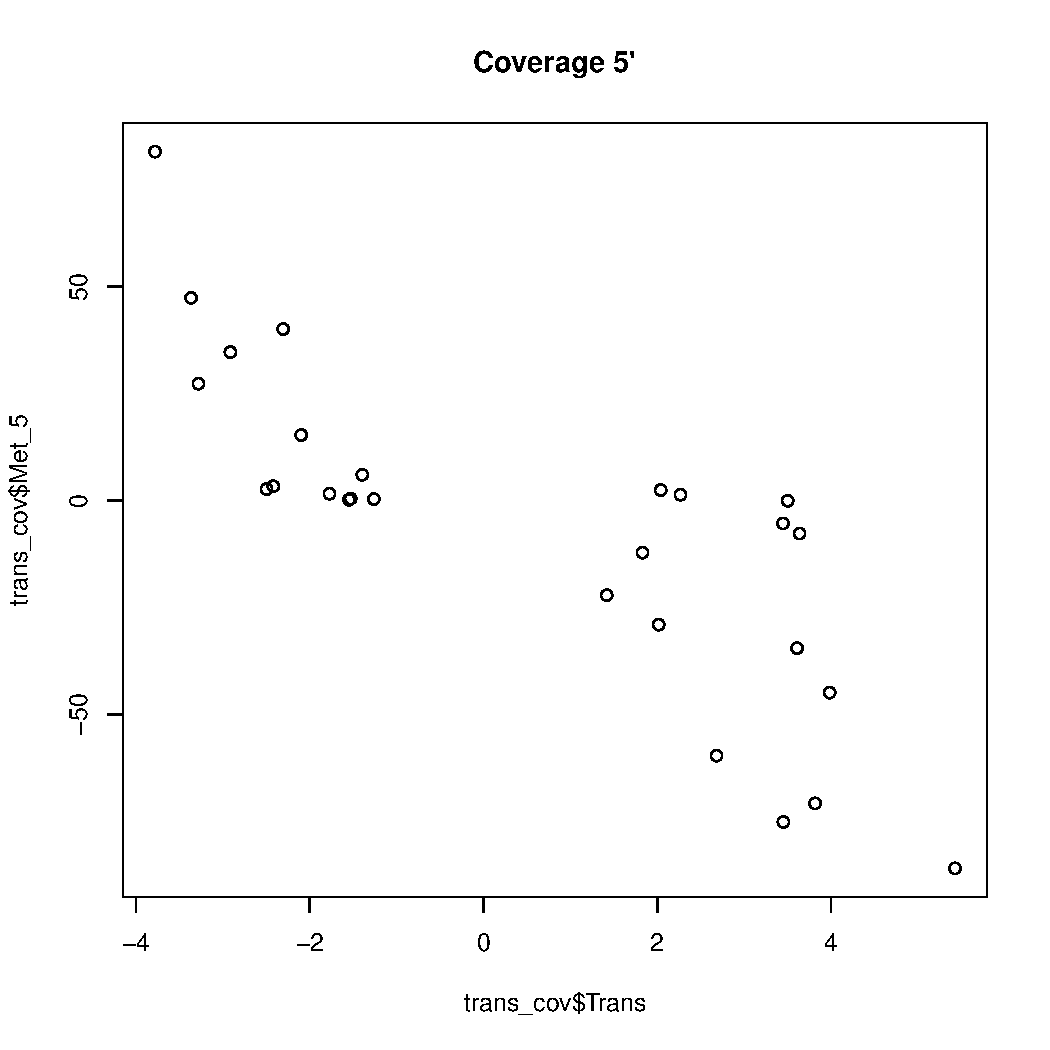
\includegraphics[width=\maxwidth]{figure/minimal-correlacions_trans-4} 
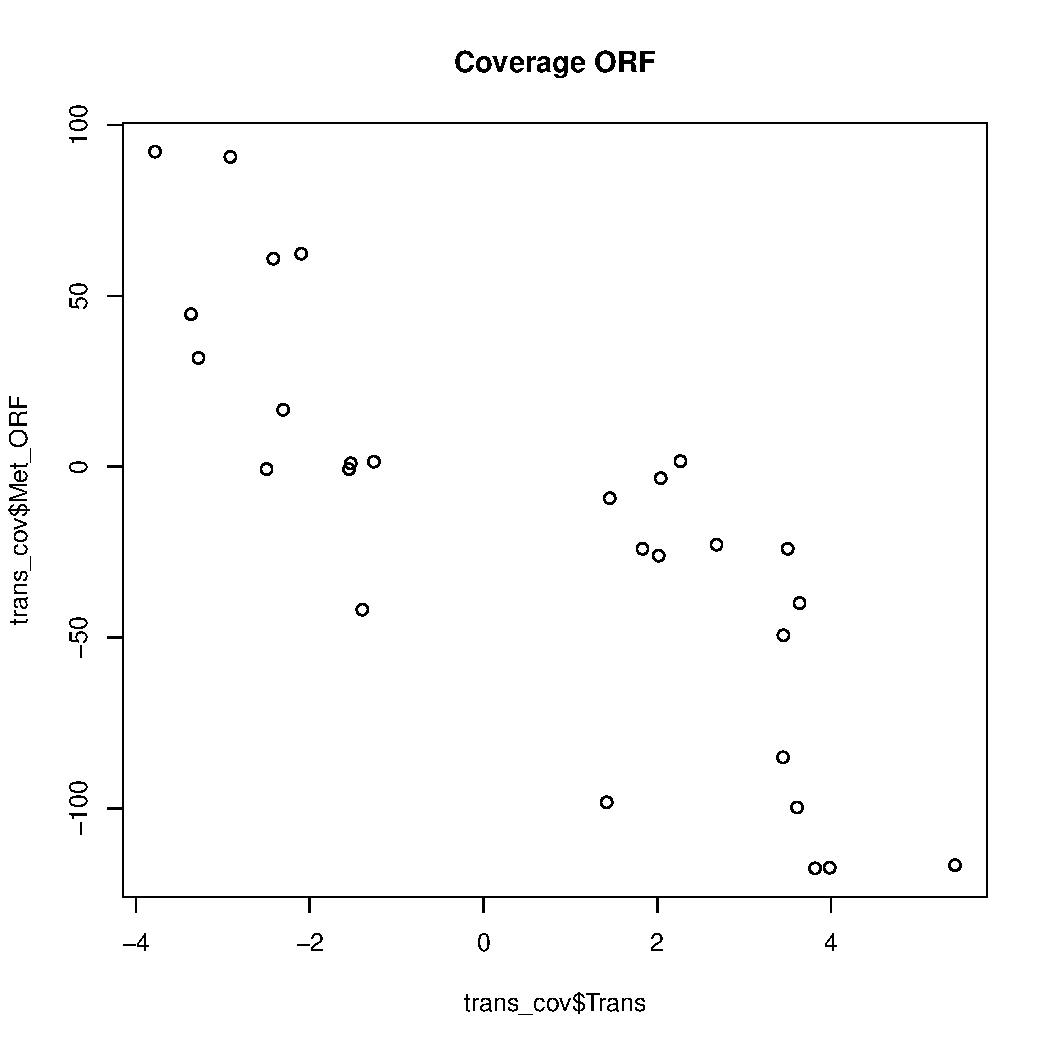
\includegraphics[width=\maxwidth]{figure/minimal-correlacions_trans-5} 
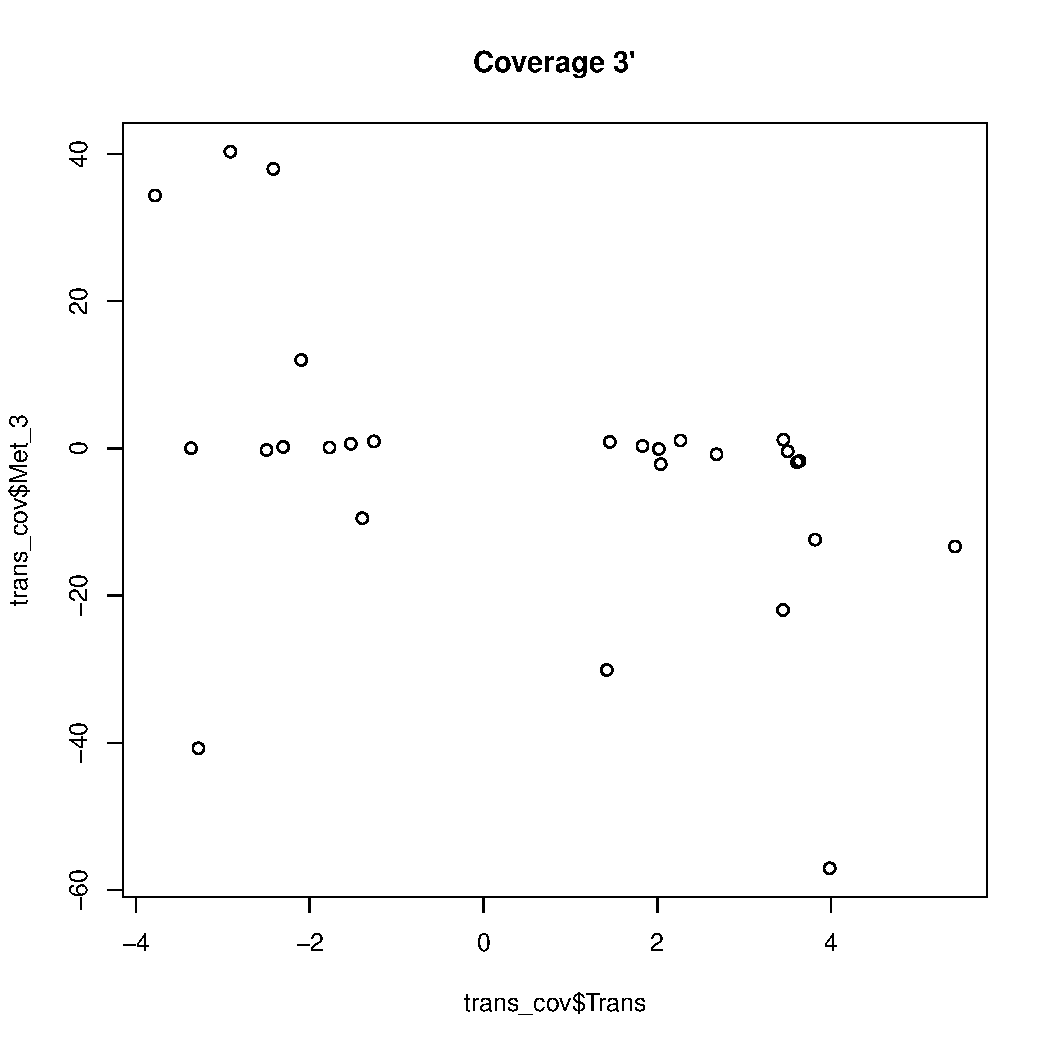
\includegraphics[width=\maxwidth]{figure/minimal-correlacions_trans-6} 
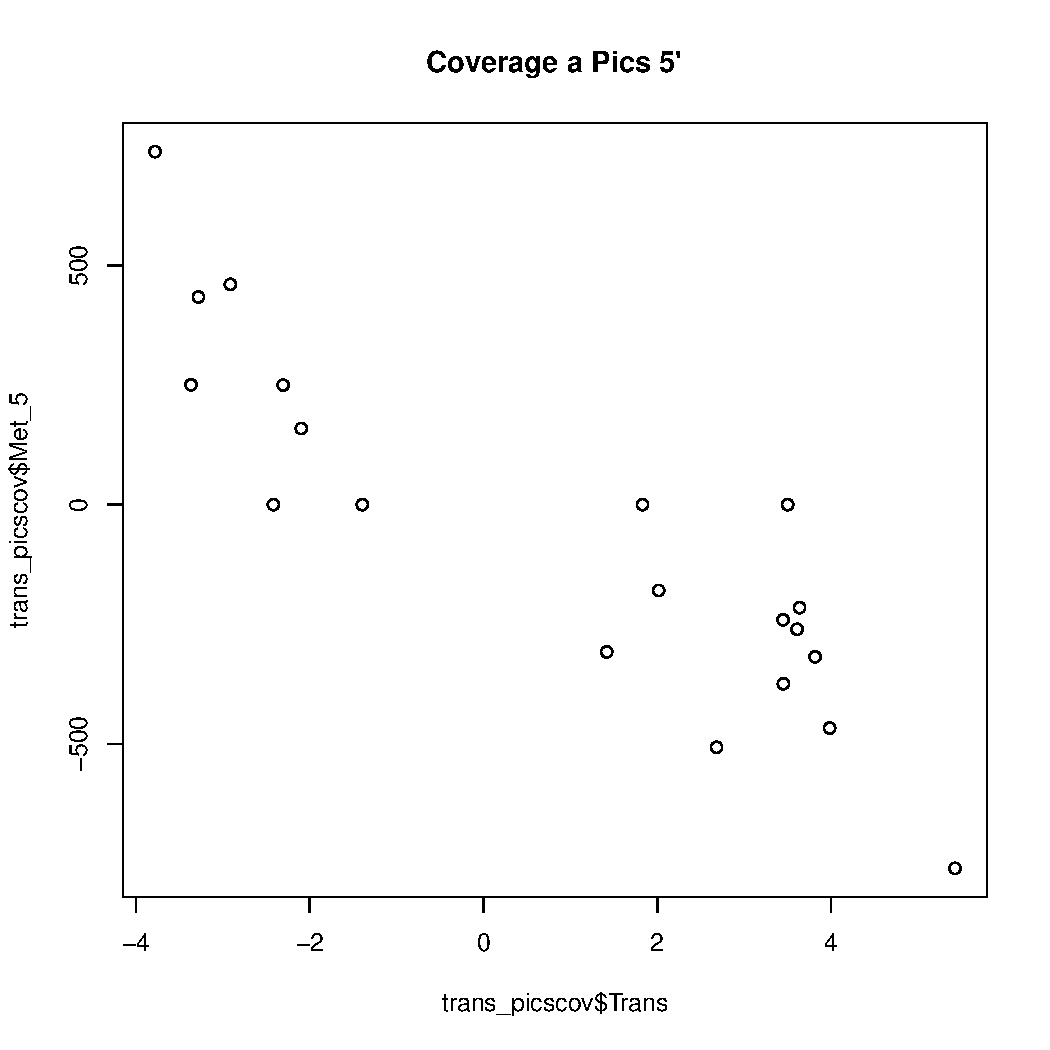
\includegraphics[width=\maxwidth]{figure/minimal-correlacions_trans-7} 
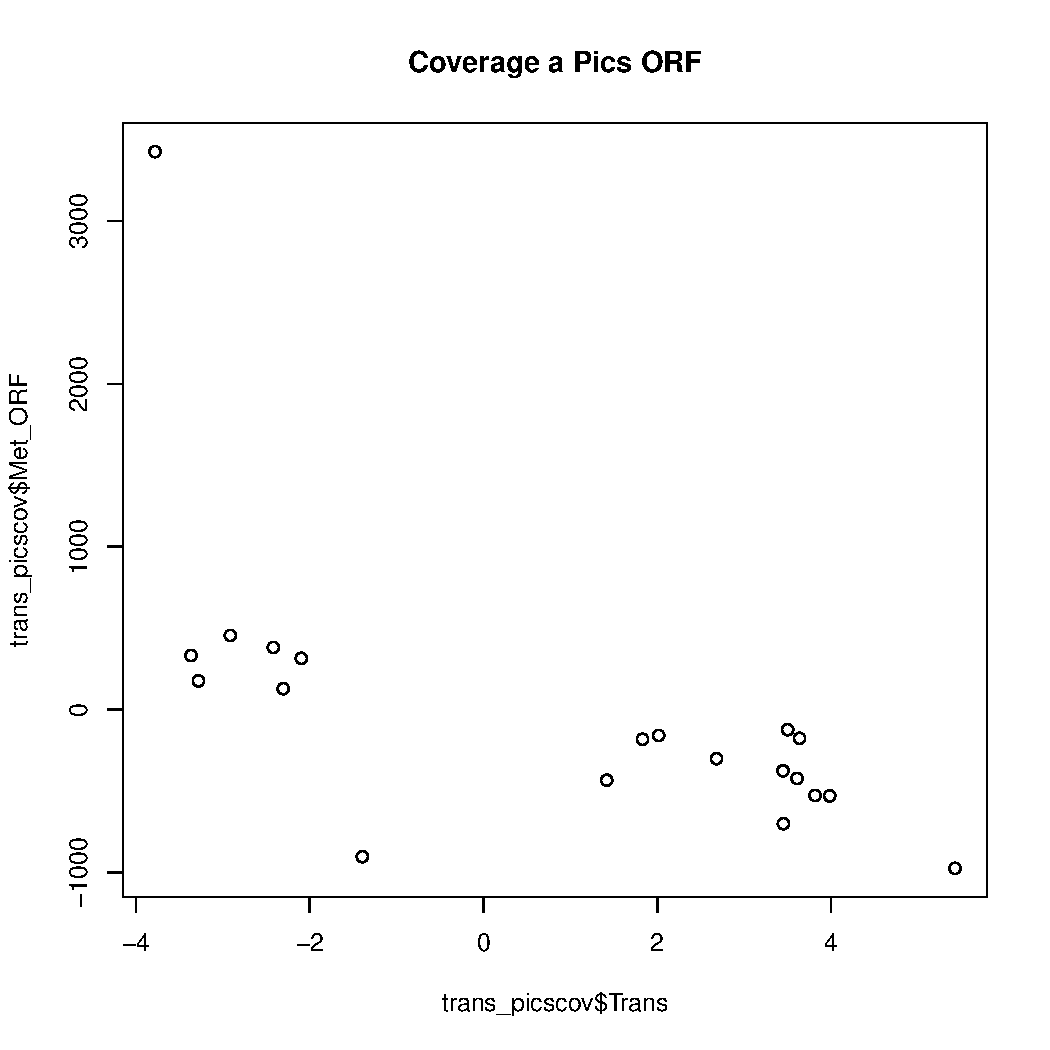
\includegraphics[width=\maxwidth]{figure/minimal-correlacions_trans-8} 
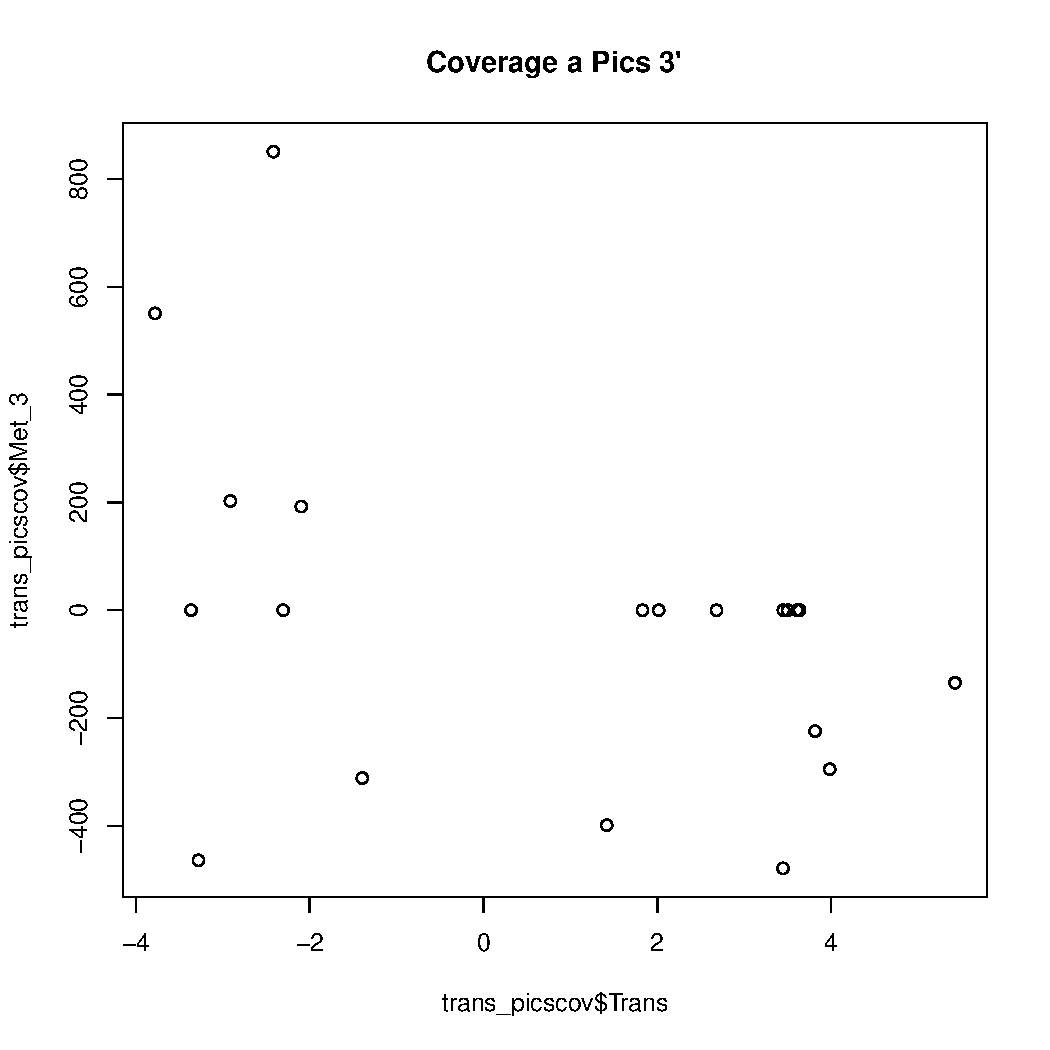
\includegraphics[width=\maxwidth]{figure/minimal-correlacions_trans-9} 

}



\end{knitrout}
\clearpage

\subsubsection{Filtrats per Metilació}
\begin{knitrout}
\definecolor{shadecolor}{rgb}{0.969, 0.969, 0.969}\color{fgcolor}

{\centering 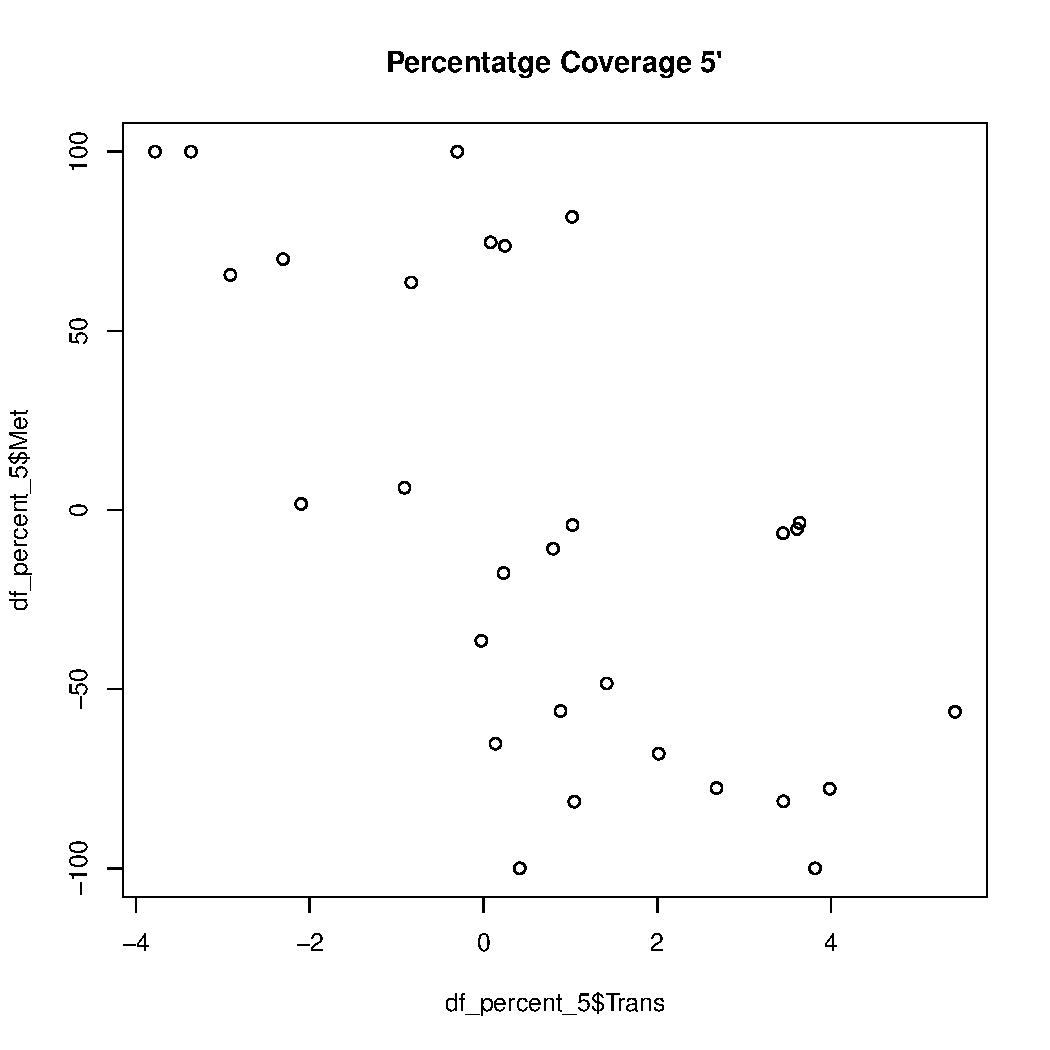
\includegraphics[width=\maxwidth]{figure/minimal-correlacions_met-1} 
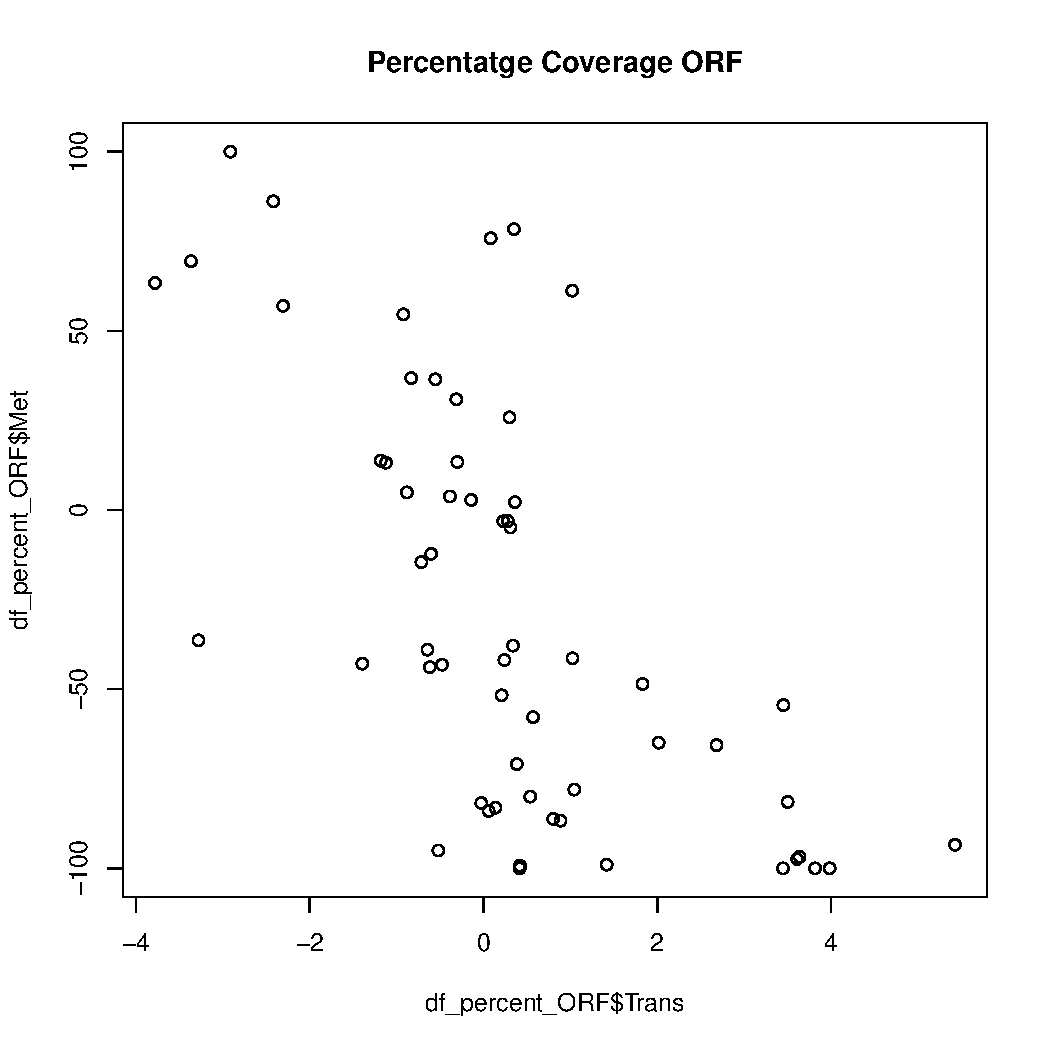
\includegraphics[width=\maxwidth]{figure/minimal-correlacions_met-2} 
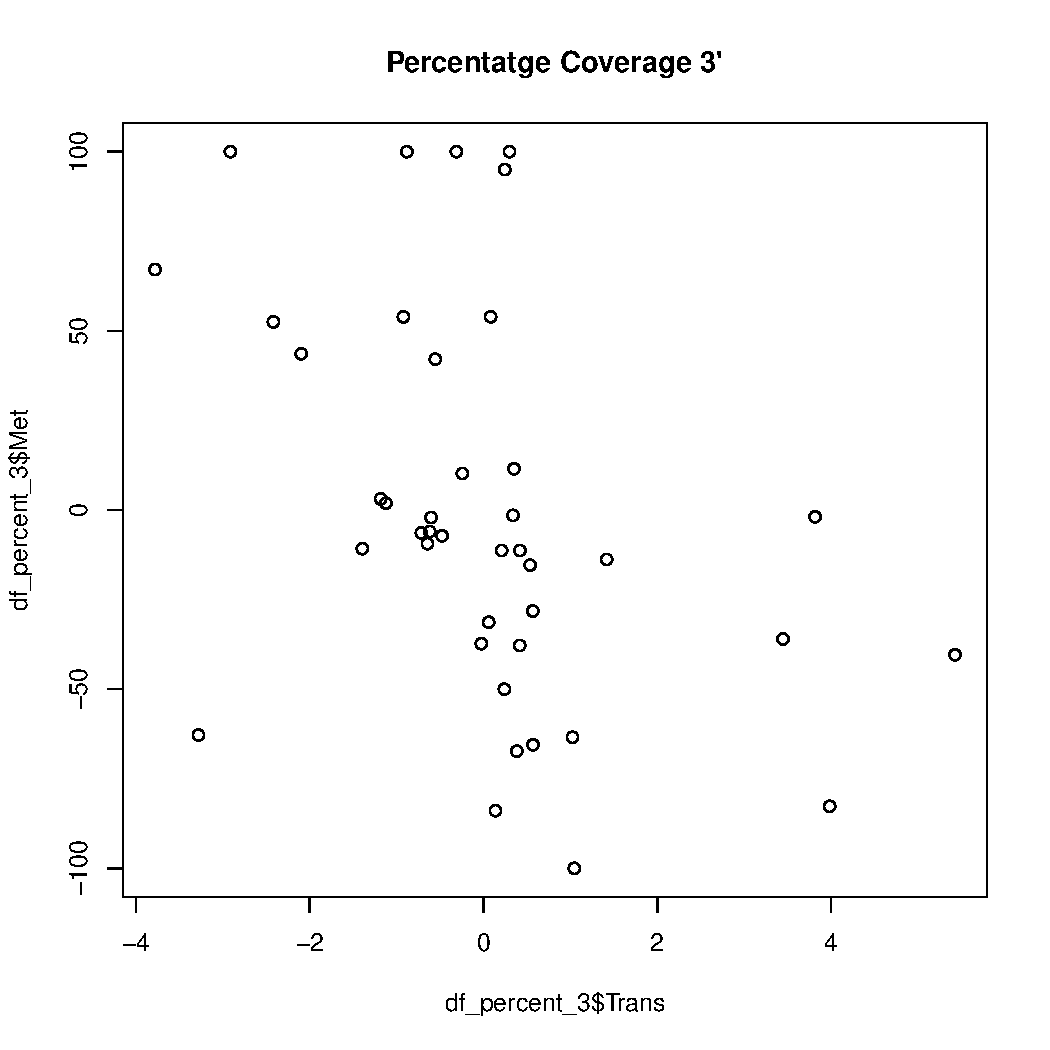
\includegraphics[width=\maxwidth]{figure/minimal-correlacions_met-3} 
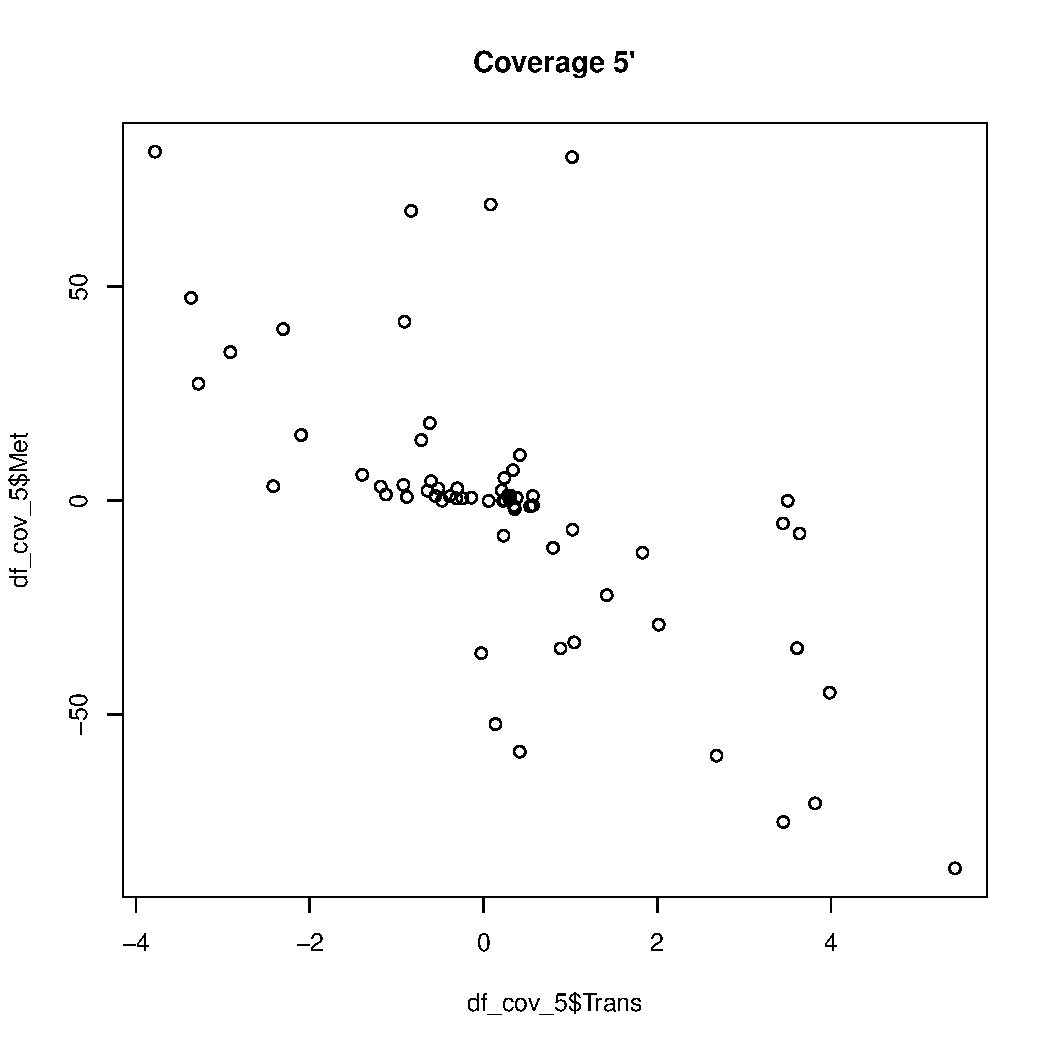
\includegraphics[width=\maxwidth]{figure/minimal-correlacions_met-4} 
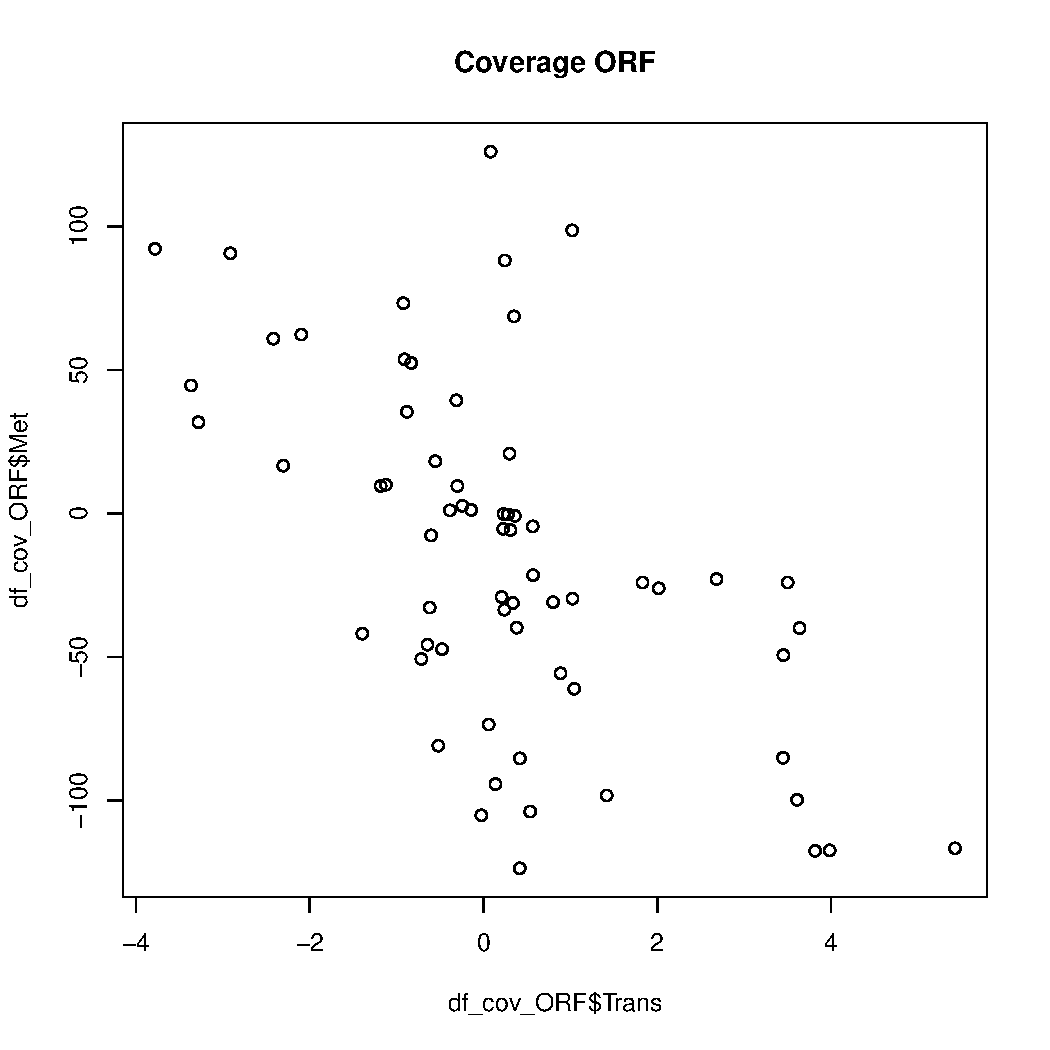
\includegraphics[width=\maxwidth]{figure/minimal-correlacions_met-5} 
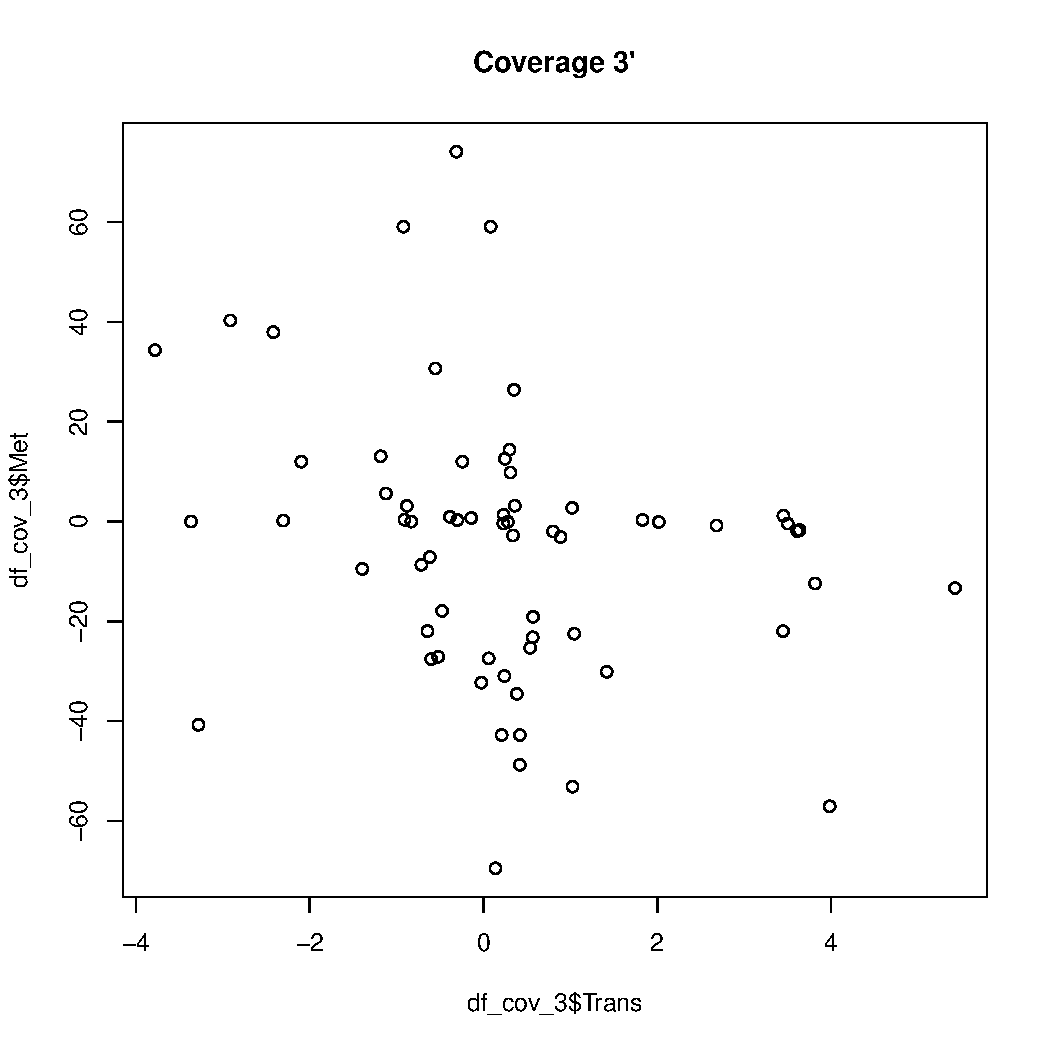
\includegraphics[width=\maxwidth]{figure/minimal-correlacions_met-6} 
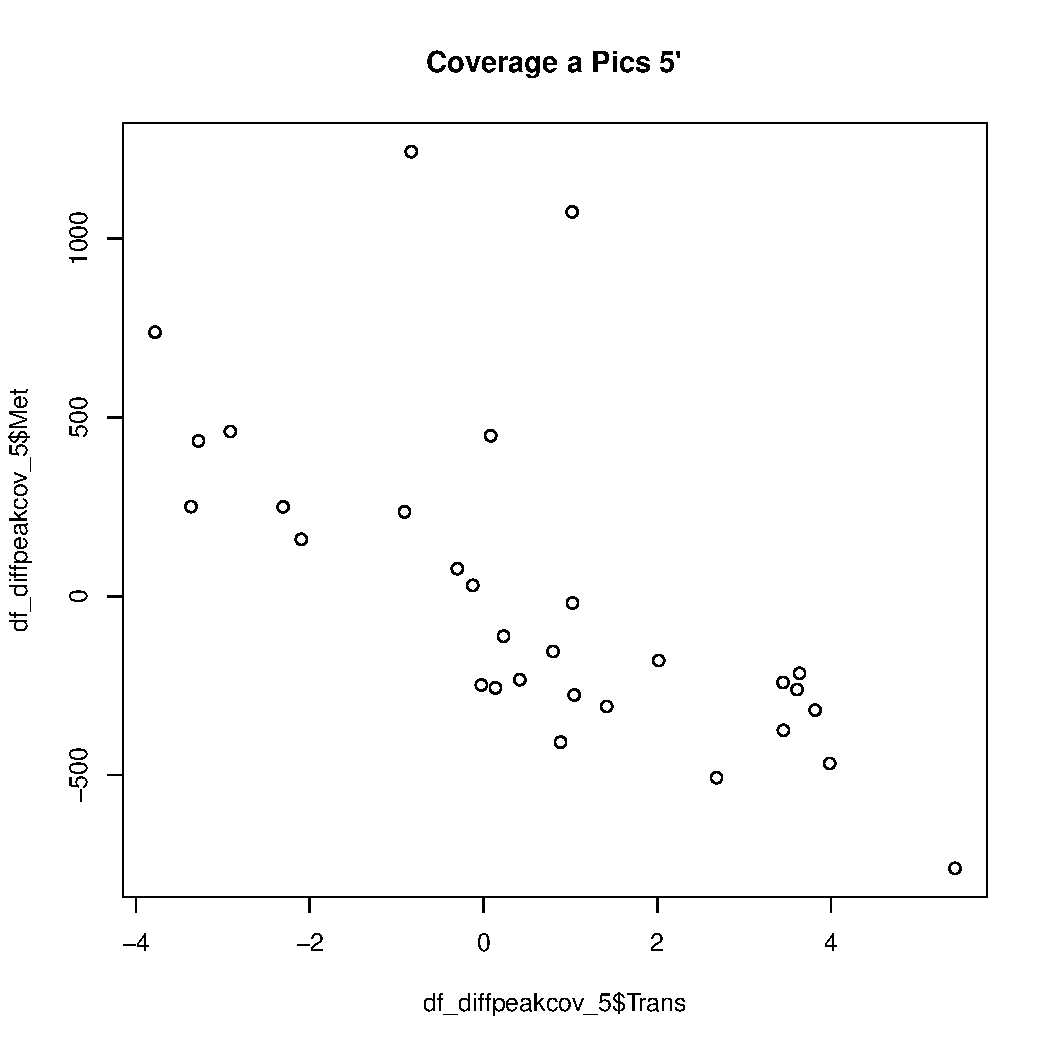
\includegraphics[width=\maxwidth]{figure/minimal-correlacions_met-7} 
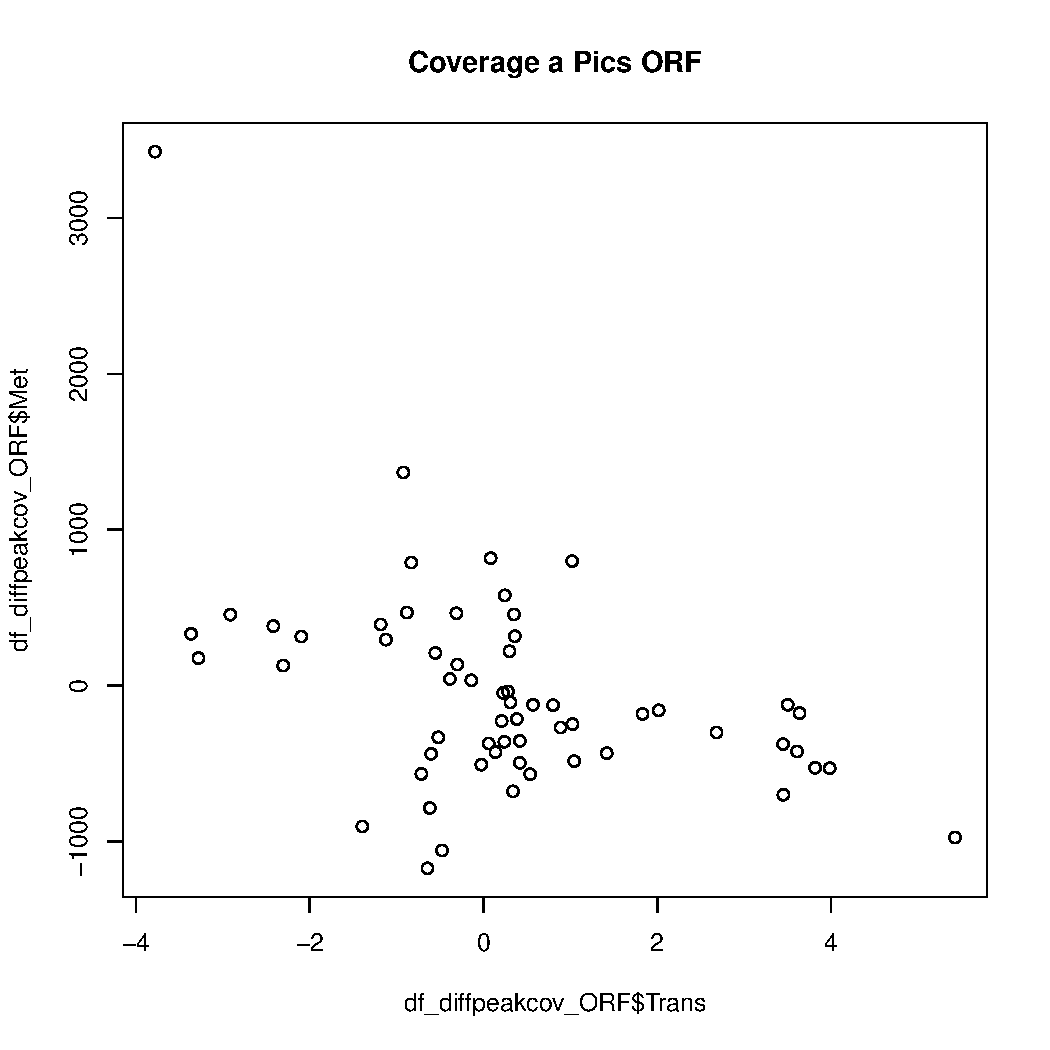
\includegraphics[width=\maxwidth]{figure/minimal-correlacions_met-8} 
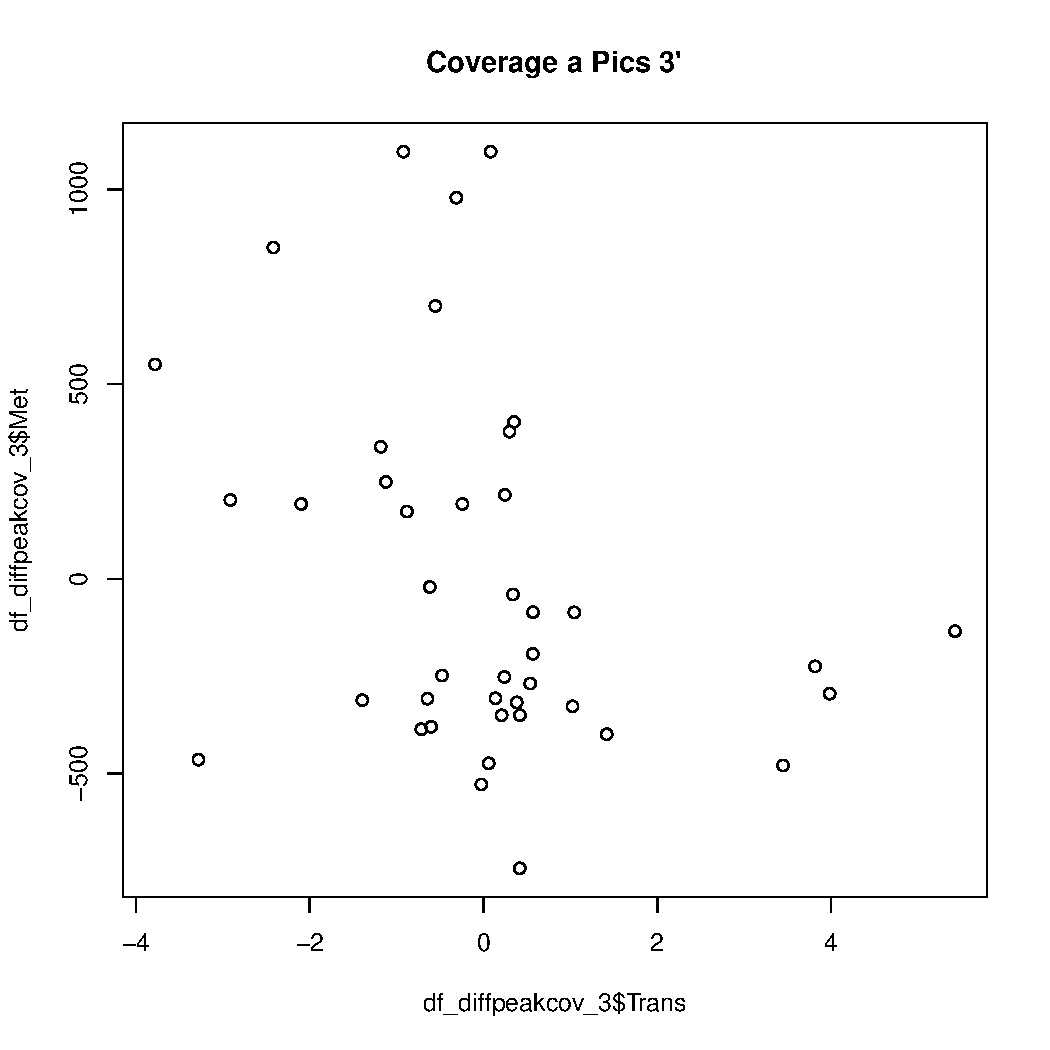
\includegraphics[width=\maxwidth]{figure/minimal-correlacions_met-9} 

}



\end{knitrout}
\clearpage

\subsection{Taula}
\subsubsection{Filtrats per Transcripció}
\begin{tabular}{ccc|ccc|ccc}
\hline
\multicolumn{3}{c}{Percentatge} &
\multicolumn{3}{c}{Coverage} &
\multicolumn{3}{c}{Coverage a Pics} \\
\cline{1-3}
\cline{4-6}
\cline{7-9}
5' & ORF & 3' & 5' & ORF & 3' & 5' & ORF & 3' \\
\hline
-0.827 & -0.865 & -0.467 & 
-0.876 & -0.847 & -0.482 & 
-0.853 & -0.764 & -0.375\\
\hline
\end{tabular} \\\\

\subsubsection{Filtrats per Metilació}
\begin{tabular}{ccc|ccc|ccc}
\hline
\multicolumn{3}{c}{Percentatge} &
\multicolumn{3}{c}{Coverage} &
\multicolumn{3}{c}{Coverage a Pics} \\
\cline{1-3}
\cline{4-6}
\cline{7-9}
5' & ORF & 3' & 5' & ORF & 3' & 5' & ORF & 3' \\
\hline
-0.659 & -0.683 & -0.543 & 
-0.749 & -0.565 & -0.352 & 
-0.786 & -0.404 & -0.324\\
\hline
\end{tabular} \\\\

\end{document}
